\documentclass[twoside]{book}

% Packages required by doxygen
\usepackage{fixltx2e}
\usepackage{calc}
\usepackage{doxygen}
\usepackage[export]{adjustbox} % also loads graphicx
\usepackage{graphicx}
\usepackage[utf8]{inputenc}
\usepackage{makeidx}
\usepackage{multicol}
\usepackage{multirow}
\PassOptionsToPackage{warn}{textcomp}
\usepackage{textcomp}
\usepackage[nointegrals]{wasysym}
\usepackage[table]{xcolor}

% Font selection
\usepackage[T1]{fontenc}
\usepackage[scaled=.90]{helvet}
\usepackage{courier}
\usepackage{amssymb}
\usepackage{sectsty}
\renewcommand{\familydefault}{\sfdefault}
\allsectionsfont{%
  \fontseries{bc}\selectfont%
  \color{darkgray}%
}
\renewcommand{\DoxyLabelFont}{%
  \fontseries{bc}\selectfont%
  \color{darkgray}%
}
\newcommand{\+}{\discretionary{\mbox{\scriptsize$\hookleftarrow$}}{}{}}

% Page & text layout
\usepackage{geometry}
\geometry{%
  a4paper,%
  top=2.5cm,%
  bottom=2.5cm,%
  left=2.5cm,%
  right=2.5cm%
}
\tolerance=750
\hfuzz=15pt
\hbadness=750
\setlength{\emergencystretch}{15pt}
\setlength{\parindent}{0cm}
\setlength{\parskip}{3ex plus 2ex minus 2ex}
\makeatletter
\renewcommand{\paragraph}{%
  \@startsection{paragraph}{4}{0ex}{-1.0ex}{1.0ex}{%
    \normalfont\normalsize\bfseries\SS@parafont%
  }%
}
\renewcommand{\subparagraph}{%
  \@startsection{subparagraph}{5}{0ex}{-1.0ex}{1.0ex}{%
    \normalfont\normalsize\bfseries\SS@subparafont%
  }%
}
\makeatother

% Headers & footers
\usepackage{fancyhdr}
\pagestyle{fancyplain}
\fancyhead[LE]{\fancyplain{}{\bfseries\thepage}}
\fancyhead[CE]{\fancyplain{}{}}
\fancyhead[RE]{\fancyplain{}{\bfseries\leftmark}}
\fancyhead[LO]{\fancyplain{}{\bfseries\rightmark}}
\fancyhead[CO]{\fancyplain{}{}}
\fancyhead[RO]{\fancyplain{}{\bfseries\thepage}}
\fancyfoot[LE]{\fancyplain{}{}}
\fancyfoot[CE]{\fancyplain{}{}}
\fancyfoot[RE]{\fancyplain{}{\bfseries\scriptsize Generated by Doxygen }}
\fancyfoot[LO]{\fancyplain{}{\bfseries\scriptsize Generated by Doxygen }}
\fancyfoot[CO]{\fancyplain{}{}}
\fancyfoot[RO]{\fancyplain{}{}}
\renewcommand{\footrulewidth}{0.4pt}
\renewcommand{\chaptermark}[1]{%
  \markboth{#1}{}%
}
\renewcommand{\sectionmark}[1]{%
  \markright{\thesection\ #1}%
}

% Indices & bibliography
\usepackage{natbib}
\usepackage[titles]{tocloft}
\setcounter{tocdepth}{3}
\setcounter{secnumdepth}{5}
\makeindex

% Hyperlinks (required, but should be loaded last)
\usepackage{ifpdf}
\ifpdf
  \usepackage[pdftex,pagebackref=true]{hyperref}
\else
  \usepackage[ps2pdf,pagebackref=true]{hyperref}
\fi
\hypersetup{%
  colorlinks=true,%
  linkcolor=blue,%
  citecolor=blue,%
  unicode%
}

% Custom commands
\newcommand{\clearemptydoublepage}{%
  \newpage{\pagestyle{empty}\cleardoublepage}%
}

\usepackage{caption}
\captionsetup{labelsep=space,justification=centering,font={bf},singlelinecheck=off,skip=4pt,position=top}

%===== C O N T E N T S =====

\begin{document}

% Titlepage & ToC
\hypersetup{pageanchor=false,
             bookmarksnumbered=true,
             pdfencoding=unicode
            }
\pagenumbering{alph}
\begin{titlepage}
\vspace*{7cm}
\begin{center}%
{\Large P\+C\+SC Monte Carlo }\\
\vspace*{1cm}
{\large Generated by Doxygen 1.8.13}\\
\end{center}
\end{titlepage}
\clearemptydoublepage
\pagenumbering{roman}
\tableofcontents
\clearemptydoublepage
\pagenumbering{arabic}
\hypersetup{pageanchor=true}

%--- Begin generated contents ---
\chapter{Hierarchical Index}
\section{Class Hierarchy}
This inheritance list is sorted roughly, but not completely, alphabetically\+:\begin{DoxyCompactList}
\item \contentsline{section}{matplotlibcpp\+:\+:detail\+:\+:\+\_\+interpreter}{\pageref{structmatplotlibcpp_1_1detail_1_1__interpreter}}{}
\item \contentsline{section}{Distribution$<$ result\+\_\+type $>$}{\pageref{class_distribution}}{}
\item \contentsline{section}{Distribution$<$ double $>$}{\pageref{class_distribution}}{}
\begin{DoxyCompactList}
\item \contentsline{section}{Exponential}{\pageref{class_exponential}}{}
\item \contentsline{section}{Normal}{\pageref{class_normal}}{}
\item \contentsline{section}{Uniform}{\pageref{class_uniform}}{}
\end{DoxyCompactList}
\item \contentsline{section}{Distribution$<$ int $>$}{\pageref{class_distribution}}{}
\begin{DoxyCompactList}
\item \contentsline{section}{Geometric}{\pageref{class_geometric}}{}
\end{DoxyCompactList}
\item \contentsline{section}{Exception}{\pageref{struct_exception}}{}
\item \contentsline{section}{Moments}{\pageref{class_moments}}{}
\item \contentsline{section}{Printer}{\pageref{struct_printer}}{}
\item \contentsline{section}{matplotlibcpp\+:\+:select\+\_\+npy\+\_\+type$<$ T $>$}{\pageref{structmatplotlibcpp_1_1select__npy__type}}{}
\item \contentsline{section}{matplotlibcpp\+:\+:select\+\_\+npy\+\_\+type$<$ bool $>$}{\pageref{structmatplotlibcpp_1_1select__npy__type_3_01bool_01_4}}{}
\item \contentsline{section}{matplotlibcpp\+:\+:select\+\_\+npy\+\_\+type$<$ double $>$}{\pageref{structmatplotlibcpp_1_1select__npy__type_3_01double_01_4}}{}
\item \contentsline{section}{matplotlibcpp\+:\+:select\+\_\+npy\+\_\+type$<$ float $>$}{\pageref{structmatplotlibcpp_1_1select__npy__type_3_01float_01_4}}{}
\item \contentsline{section}{matplotlibcpp\+:\+:select\+\_\+npy\+\_\+type$<$ int16\+\_\+t $>$}{\pageref{structmatplotlibcpp_1_1select__npy__type_3_01int16__t_01_4}}{}
\item \contentsline{section}{matplotlibcpp\+:\+:select\+\_\+npy\+\_\+type$<$ int32\+\_\+t $>$}{\pageref{structmatplotlibcpp_1_1select__npy__type_3_01int32__t_01_4}}{}
\item \contentsline{section}{matplotlibcpp\+:\+:select\+\_\+npy\+\_\+type$<$ int64\+\_\+t $>$}{\pageref{structmatplotlibcpp_1_1select__npy__type_3_01int64__t_01_4}}{}
\item \contentsline{section}{matplotlibcpp\+:\+:select\+\_\+npy\+\_\+type$<$ int8\+\_\+t $>$}{\pageref{structmatplotlibcpp_1_1select__npy__type_3_01int8__t_01_4}}{}
\item \contentsline{section}{matplotlibcpp\+:\+:select\+\_\+npy\+\_\+type$<$ uint16\+\_\+t $>$}{\pageref{structmatplotlibcpp_1_1select__npy__type_3_01uint16__t_01_4}}{}
\item \contentsline{section}{matplotlibcpp\+:\+:select\+\_\+npy\+\_\+type$<$ uint32\+\_\+t $>$}{\pageref{structmatplotlibcpp_1_1select__npy__type_3_01uint32__t_01_4}}{}
\item \contentsline{section}{matplotlibcpp\+:\+:select\+\_\+npy\+\_\+type$<$ uint64\+\_\+t $>$}{\pageref{structmatplotlibcpp_1_1select__npy__type_3_01uint64__t_01_4}}{}
\item \contentsline{section}{matplotlibcpp\+:\+:select\+\_\+npy\+\_\+type$<$ uint8\+\_\+t $>$}{\pageref{structmatplotlibcpp_1_1select__npy__type_3_01uint8__t_01_4}}{}
\item \contentsline{section}{Verify\+C\+LT}{\pageref{class_verify_c_l_t}}{}
\end{DoxyCompactList}

\chapter{Class Index}
\section{Class List}
Here are the classes, structs, unions and interfaces with brief descriptions\+:\begin{DoxyCompactList}
\item\contentsline{section}{\hyperlink{classgnuplotio_1_1ArrayTraits}{gnuplotio\+::\+Array\+Traits$<$ T, Enable $>$} }{\pageref{classgnuplotio_1_1ArrayTraits}}{}
\item\contentsline{section}{\hyperlink{classgnuplotio_1_1ArrayTraits_3_01std_1_1pair_3_01T_00_01U_01_4_01_4}{gnuplotio\+::\+Array\+Traits$<$ std\+::pair$<$ T, U $>$ $>$} }{\pageref{classgnuplotio_1_1ArrayTraits_3_01std_1_1pair_3_01T_00_01U_01_4_01_4}}{}
\item\contentsline{section}{\hyperlink{classgnuplotio_1_1ArrayTraits_3_01T_01_6_01_4}{gnuplotio\+::\+Array\+Traits$<$ T \& $>$} }{\pageref{classgnuplotio_1_1ArrayTraits_3_01T_01_6_01_4}}{}
\item\contentsline{section}{\hyperlink{classgnuplotio_1_1ArrayTraits_3_01T_00_01typename_01boost_1_1enable__if_3_01boost_1_1mpl_1_1and_371638f7d82cde4b7a8a064d0797371a}{gnuplotio\+::\+Array\+Traits$<$ T, typename boost\+::enable\+\_\+if$<$ boost\+::mpl\+::and\+\_\+$<$ is\+\_\+boost\+\_\+tuple$<$ T $>$, boost\+::mpl\+::not\+\_\+$<$ is\+\_\+boost\+\_\+tuple\+\_\+nulltype$<$ typename T\+::tail\+\_\+type $>$ $>$ $>$ $>$\+::type $>$} }{\pageref{classgnuplotio_1_1ArrayTraits_3_01T_00_01typename_01boost_1_1enable__if_3_01boost_1_1mpl_1_1and_371638f7d82cde4b7a8a064d0797371a}}{}
\item\contentsline{section}{\hyperlink{classgnuplotio_1_1ArrayTraits_3_01T_00_01typename_01boost_1_1enable__if_3_01boost_1_1mpl_1_1and_d5bfbd58f322d0a74d370034dff1881d}{gnuplotio\+::\+Array\+Traits$<$ T, typename boost\+::enable\+\_\+if$<$ boost\+::mpl\+::and\+\_\+$<$ is\+\_\+boost\+\_\+tuple$<$ T $>$, is\+\_\+boost\+\_\+tuple\+\_\+nulltype$<$ typename T\+::tail\+\_\+type $>$ $>$ $>$\+::type $>$} }{\pageref{classgnuplotio_1_1ArrayTraits_3_01T_00_01typename_01boost_1_1enable__if_3_01boost_1_1mpl_1_1and_d5bfbd58f322d0a74d370034dff1881d}}{}
\item\contentsline{section}{\hyperlink{classgnuplotio_1_1ArrayTraits_3_01T_00_01typename_01boost_1_1enable__if_3_01is__like__stl__conta99f8c9e80e271bc1ed047cdd05794af4}{gnuplotio\+::\+Array\+Traits$<$ T, typename boost\+::enable\+\_\+if$<$ is\+\_\+like\+\_\+stl\+\_\+container$<$ T $>$ $>$\+::type $>$} }{\pageref{classgnuplotio_1_1ArrayTraits_3_01T_00_01typename_01boost_1_1enable__if_3_01is__like__stl__conta99f8c9e80e271bc1ed047cdd05794af4}}{}
\item\contentsline{section}{\hyperlink{classgnuplotio_1_1ArrayTraits_3_01T[N]_4}{gnuplotio\+::\+Array\+Traits$<$ T\mbox{[}\+N\mbox{]}$>$} }{\pageref{classgnuplotio_1_1ArrayTraits_3_01T[N]_4}}{}
\item\contentsline{section}{\hyperlink{classgnuplotio_1_1ArrayTraitsDefaults}{gnuplotio\+::\+Array\+Traits\+Defaults$<$ V $>$} }{\pageref{classgnuplotio_1_1ArrayTraitsDefaults}}{}
\item\contentsline{section}{\hyperlink{structgnuplotio_1_1BinarySender}{gnuplotio\+::\+Binary\+Sender$<$ T, Enable $>$} }{\pageref{structgnuplotio_1_1BinarySender}}{}
\item\contentsline{section}{\hyperlink{structgnuplotio_1_1BinarySender_3_01boost_1_1int16__t_01_4}{gnuplotio\+::\+Binary\+Sender$<$ boost\+::int16\+\_\+t $>$} }{\pageref{structgnuplotio_1_1BinarySender_3_01boost_1_1int16__t_01_4}}{}
\item\contentsline{section}{\hyperlink{structgnuplotio_1_1BinarySender_3_01boost_1_1int32__t_01_4}{gnuplotio\+::\+Binary\+Sender$<$ boost\+::int32\+\_\+t $>$} }{\pageref{structgnuplotio_1_1BinarySender_3_01boost_1_1int32__t_01_4}}{}
\item\contentsline{section}{\hyperlink{structgnuplotio_1_1BinarySender_3_01boost_1_1int64__t_01_4}{gnuplotio\+::\+Binary\+Sender$<$ boost\+::int64\+\_\+t $>$} }{\pageref{structgnuplotio_1_1BinarySender_3_01boost_1_1int64__t_01_4}}{}
\item\contentsline{section}{\hyperlink{structgnuplotio_1_1BinarySender_3_01boost_1_1int8__t_01_4}{gnuplotio\+::\+Binary\+Sender$<$ boost\+::int8\+\_\+t $>$} }{\pageref{structgnuplotio_1_1BinarySender_3_01boost_1_1int8__t_01_4}}{}
\item\contentsline{section}{\hyperlink{structgnuplotio_1_1BinarySender_3_01boost_1_1uint16__t_01_4}{gnuplotio\+::\+Binary\+Sender$<$ boost\+::uint16\+\_\+t $>$} }{\pageref{structgnuplotio_1_1BinarySender_3_01boost_1_1uint16__t_01_4}}{}
\item\contentsline{section}{\hyperlink{structgnuplotio_1_1BinarySender_3_01boost_1_1uint32__t_01_4}{gnuplotio\+::\+Binary\+Sender$<$ boost\+::uint32\+\_\+t $>$} }{\pageref{structgnuplotio_1_1BinarySender_3_01boost_1_1uint32__t_01_4}}{}
\item\contentsline{section}{\hyperlink{structgnuplotio_1_1BinarySender_3_01boost_1_1uint64__t_01_4}{gnuplotio\+::\+Binary\+Sender$<$ boost\+::uint64\+\_\+t $>$} }{\pageref{structgnuplotio_1_1BinarySender_3_01boost_1_1uint64__t_01_4}}{}
\item\contentsline{section}{\hyperlink{structgnuplotio_1_1BinarySender_3_01boost_1_1uint8__t_01_4}{gnuplotio\+::\+Binary\+Sender$<$ boost\+::uint8\+\_\+t $>$} }{\pageref{structgnuplotio_1_1BinarySender_3_01boost_1_1uint8__t_01_4}}{}
\item\contentsline{section}{\hyperlink{structgnuplotio_1_1BinarySender_3_01double_01_4}{gnuplotio\+::\+Binary\+Sender$<$ double $>$} }{\pageref{structgnuplotio_1_1BinarySender_3_01double_01_4}}{}
\item\contentsline{section}{\hyperlink{structgnuplotio_1_1BinarySender_3_01float_01_4}{gnuplotio\+::\+Binary\+Sender$<$ float $>$} }{\pageref{structgnuplotio_1_1BinarySender_3_01float_01_4}}{}
\item\contentsline{section}{\hyperlink{structgnuplotio_1_1BinarySender_3_01std_1_1complex_3_01T_01_4_01_4}{gnuplotio\+::\+Binary\+Sender$<$ std\+::complex$<$ T $>$ $>$} }{\pageref{structgnuplotio_1_1BinarySender_3_01std_1_1complex_3_01T_01_4_01_4}}{}
\item\contentsline{section}{\hyperlink{structgnuplotio_1_1BinarySender_3_01std_1_1pair_3_01T_00_01U_01_4_01_4}{gnuplotio\+::\+Binary\+Sender$<$ std\+::pair$<$ T, U $>$ $>$} }{\pageref{structgnuplotio_1_1BinarySender_3_01std_1_1pair_3_01T_00_01U_01_4_01_4}}{}
\item\contentsline{section}{\hyperlink{structgnuplotio_1_1BinarySender_3_01T_00_01typename_01boost_1_1enable__if_3_01boost_1_1mpl_1_1anab84516ea337555045555dbce2b6c996}{gnuplotio\+::\+Binary\+Sender$<$ T, typename boost\+::enable\+\_\+if$<$ boost\+::mpl\+::and\+\_\+$<$ is\+\_\+boost\+\_\+tuple$<$ T $>$, boost\+::mpl\+::not\+\_\+$<$ is\+\_\+boost\+\_\+tuple\+\_\+nulltype$<$ typename T\+::tail\+\_\+type $>$ $>$ $>$ $>$\+::type $>$} }{\pageref{structgnuplotio_1_1BinarySender_3_01T_00_01typename_01boost_1_1enable__if_3_01boost_1_1mpl_1_1anab84516ea337555045555dbce2b6c996}}{}
\item\contentsline{section}{\hyperlink{structgnuplotio_1_1BinarySender_3_01T_00_01typename_01boost_1_1enable__if_3_01boost_1_1mpl_1_1anbc7c19c30874558f14f1e5020da805a3}{gnuplotio\+::\+Binary\+Sender$<$ T, typename boost\+::enable\+\_\+if$<$ boost\+::mpl\+::and\+\_\+$<$ is\+\_\+boost\+\_\+tuple$<$ T $>$, is\+\_\+boost\+\_\+tuple\+\_\+nulltype$<$ typename T\+::tail\+\_\+type $>$ $>$ $>$\+::type $>$} }{\pageref{structgnuplotio_1_1BinarySender_3_01T_00_01typename_01boost_1_1enable__if_3_01boost_1_1mpl_1_1anbc7c19c30874558f14f1e5020da805a3}}{}
\item\contentsline{section}{\hyperlink{structgnuplotio_1_1BinfmtSender}{gnuplotio\+::\+Binfmt\+Sender$<$ T, Enable $>$} }{\pageref{structgnuplotio_1_1BinfmtSender}}{}
\item\contentsline{section}{\hyperlink{structgnuplotio_1_1BinfmtSender_3_01boost_1_1int16__t_01_4}{gnuplotio\+::\+Binfmt\+Sender$<$ boost\+::int16\+\_\+t $>$} }{\pageref{structgnuplotio_1_1BinfmtSender_3_01boost_1_1int16__t_01_4}}{}
\item\contentsline{section}{\hyperlink{structgnuplotio_1_1BinfmtSender_3_01boost_1_1int32__t_01_4}{gnuplotio\+::\+Binfmt\+Sender$<$ boost\+::int32\+\_\+t $>$} }{\pageref{structgnuplotio_1_1BinfmtSender_3_01boost_1_1int32__t_01_4}}{}
\item\contentsline{section}{\hyperlink{structgnuplotio_1_1BinfmtSender_3_01boost_1_1int64__t_01_4}{gnuplotio\+::\+Binfmt\+Sender$<$ boost\+::int64\+\_\+t $>$} }{\pageref{structgnuplotio_1_1BinfmtSender_3_01boost_1_1int64__t_01_4}}{}
\item\contentsline{section}{\hyperlink{structgnuplotio_1_1BinfmtSender_3_01boost_1_1int8__t_01_4}{gnuplotio\+::\+Binfmt\+Sender$<$ boost\+::int8\+\_\+t $>$} }{\pageref{structgnuplotio_1_1BinfmtSender_3_01boost_1_1int8__t_01_4}}{}
\item\contentsline{section}{\hyperlink{structgnuplotio_1_1BinfmtSender_3_01boost_1_1uint16__t_01_4}{gnuplotio\+::\+Binfmt\+Sender$<$ boost\+::uint16\+\_\+t $>$} }{\pageref{structgnuplotio_1_1BinfmtSender_3_01boost_1_1uint16__t_01_4}}{}
\item\contentsline{section}{\hyperlink{structgnuplotio_1_1BinfmtSender_3_01boost_1_1uint32__t_01_4}{gnuplotio\+::\+Binfmt\+Sender$<$ boost\+::uint32\+\_\+t $>$} }{\pageref{structgnuplotio_1_1BinfmtSender_3_01boost_1_1uint32__t_01_4}}{}
\item\contentsline{section}{\hyperlink{structgnuplotio_1_1BinfmtSender_3_01boost_1_1uint64__t_01_4}{gnuplotio\+::\+Binfmt\+Sender$<$ boost\+::uint64\+\_\+t $>$} }{\pageref{structgnuplotio_1_1BinfmtSender_3_01boost_1_1uint64__t_01_4}}{}
\item\contentsline{section}{\hyperlink{structgnuplotio_1_1BinfmtSender_3_01boost_1_1uint8__t_01_4}{gnuplotio\+::\+Binfmt\+Sender$<$ boost\+::uint8\+\_\+t $>$} }{\pageref{structgnuplotio_1_1BinfmtSender_3_01boost_1_1uint8__t_01_4}}{}
\item\contentsline{section}{\hyperlink{structgnuplotio_1_1BinfmtSender_3_01double_01_4}{gnuplotio\+::\+Binfmt\+Sender$<$ double $>$} }{\pageref{structgnuplotio_1_1BinfmtSender_3_01double_01_4}}{}
\item\contentsline{section}{\hyperlink{structgnuplotio_1_1BinfmtSender_3_01float_01_4}{gnuplotio\+::\+Binfmt\+Sender$<$ float $>$} }{\pageref{structgnuplotio_1_1BinfmtSender_3_01float_01_4}}{}
\item\contentsline{section}{\hyperlink{structgnuplotio_1_1BinfmtSender_3_01std_1_1complex_3_01T_01_4_01_4}{gnuplotio\+::\+Binfmt\+Sender$<$ std\+::complex$<$ T $>$ $>$} }{\pageref{structgnuplotio_1_1BinfmtSender_3_01std_1_1complex_3_01T_01_4_01_4}}{}
\item\contentsline{section}{\hyperlink{structgnuplotio_1_1BinfmtSender_3_01std_1_1pair_3_01T_00_01U_01_4_01_4}{gnuplotio\+::\+Binfmt\+Sender$<$ std\+::pair$<$ T, U $>$ $>$} }{\pageref{structgnuplotio_1_1BinfmtSender_3_01std_1_1pair_3_01T_00_01U_01_4_01_4}}{}
\item\contentsline{section}{\hyperlink{structgnuplotio_1_1BinfmtSender_3_01T_00_01typename_01boost_1_1enable__if_3_01boost_1_1mpl_1_1an42b95f03faee3ff44b47c946e1ea6e52}{gnuplotio\+::\+Binfmt\+Sender$<$ T, typename boost\+::enable\+\_\+if$<$ boost\+::mpl\+::and\+\_\+$<$ is\+\_\+boost\+\_\+tuple$<$ T $>$, boost\+::mpl\+::not\+\_\+$<$ is\+\_\+boost\+\_\+tuple\+\_\+nulltype$<$ typename T\+::tail\+\_\+type $>$ $>$ $>$ $>$\+::type $>$} }{\pageref{structgnuplotio_1_1BinfmtSender_3_01T_00_01typename_01boost_1_1enable__if_3_01boost_1_1mpl_1_1an42b95f03faee3ff44b47c946e1ea6e52}}{}
\item\contentsline{section}{\hyperlink{structgnuplotio_1_1BinfmtSender_3_01T_00_01typename_01boost_1_1enable__if_3_01boost_1_1mpl_1_1an36b5089f0cb57748545b30004479b7ea}{gnuplotio\+::\+Binfmt\+Sender$<$ T, typename boost\+::enable\+\_\+if$<$ boost\+::mpl\+::and\+\_\+$<$ is\+\_\+boost\+\_\+tuple$<$ T $>$, is\+\_\+boost\+\_\+tuple\+\_\+nulltype$<$ typename T\+::tail\+\_\+type $>$ $>$ $>$\+::type $>$} }{\pageref{structgnuplotio_1_1BinfmtSender_3_01T_00_01typename_01boost_1_1enable__if_3_01boost_1_1mpl_1_1an36b5089f0cb57748545b30004479b7ea}}{}
\item\contentsline{section}{\hyperlink{structgnuplotio_1_1CastIntTextSender}{gnuplotio\+::\+Cast\+Int\+Text\+Sender$<$ T $>$} }{\pageref{structgnuplotio_1_1CastIntTextSender}}{}
\item\contentsline{section}{\hyperlink{structgnuplotio_1_1ColUnwrapNo}{gnuplotio\+::\+Col\+Unwrap\+No} }{\pageref{structgnuplotio_1_1ColUnwrapNo}}{}
\item\contentsline{section}{\hyperlink{structgnuplotio_1_1ColUnwrapYes}{gnuplotio\+::\+Col\+Unwrap\+Yes} }{\pageref{structgnuplotio_1_1ColUnwrapYes}}{}
\item\contentsline{section}{\hyperlink{classDistribution}{Distribution} }{\pageref{classDistribution}}{}
\item\contentsline{section}{\hyperlink{structgnuplotio_1_1dont__treat__as__stl__container}{gnuplotio\+::dont\+\_\+treat\+\_\+as\+\_\+stl\+\_\+container$<$ T $>$} }{\pageref{structgnuplotio_1_1dont__treat__as__stl__container}}{}
\item\contentsline{section}{\hyperlink{structgnuplotio_1_1Error__InappropriateDeref}{gnuplotio\+::\+Error\+\_\+\+Inappropriate\+Deref} }{\pageref{structgnuplotio_1_1Error__InappropriateDeref}}{}
\item\contentsline{section}{\hyperlink{structgnuplotio_1_1Error__WasNotContainer}{gnuplotio\+::\+Error\+\_\+\+Was\+Not\+Container} }{\pageref{structgnuplotio_1_1Error__WasNotContainer}}{}
\item\contentsline{section}{\hyperlink{structException}{Exception} }{\pageref{structException}}{}
\item\contentsline{section}{\hyperlink{classExpectation}{Expectation} }{\pageref{classExpectation}}{}
\item\contentsline{section}{\hyperlink{classExponential}{Exponential} }{\pageref{classExponential}}{}
\item\contentsline{section}{\hyperlink{structgnuplotio_1_1FileHandleWrapper}{gnuplotio\+::\+File\+Handle\+Wrapper} }{\pageref{structgnuplotio_1_1FileHandleWrapper}}{}
\item\contentsline{section}{\hyperlink{structgnuplotio_1_1FlatBinarySender}{gnuplotio\+::\+Flat\+Binary\+Sender$<$ T $>$} }{\pageref{structgnuplotio_1_1FlatBinarySender}}{}
\item\contentsline{section}{\hyperlink{structgnuplotio_1_1FloatTextSender}{gnuplotio\+::\+Float\+Text\+Sender$<$ T $>$} }{\pageref{structgnuplotio_1_1FloatTextSender}}{}
\item\contentsline{section}{\hyperlink{classGeometric}{Geometric} }{\pageref{classGeometric}}{}
\item\contentsline{section}{\hyperlink{classgnuplotio_1_1Gnuplot}{gnuplotio\+::\+Gnuplot} }{\pageref{classgnuplotio_1_1Gnuplot}}{}
\item\contentsline{section}{\hyperlink{classgnuplotio_1_1GnuplotFeedback}{gnuplotio\+::\+Gnuplot\+Feedback} }{\pageref{classgnuplotio_1_1GnuplotFeedback}}{}
\item\contentsline{section}{\hyperlink{structgnuplotio_1_1is__boost__tuple}{gnuplotio\+::is\+\_\+boost\+\_\+tuple$<$ T $>$} }{\pageref{structgnuplotio_1_1is__boost__tuple}}{}
\item\contentsline{section}{\hyperlink{structgnuplotio_1_1is__boost__tuple__nulltype}{gnuplotio\+::is\+\_\+boost\+\_\+tuple\+\_\+nulltype$<$ T $>$} }{\pageref{structgnuplotio_1_1is__boost__tuple__nulltype}}{}
\item\contentsline{section}{\hyperlink{structgnuplotio_1_1is__boost__tuple__nulltype_3_01boost_1_1tuples_1_1null__type_01_4}{gnuplotio\+::is\+\_\+boost\+\_\+tuple\+\_\+nulltype$<$ boost\+::tuples\+::null\+\_\+type $>$} }{\pageref{structgnuplotio_1_1is__boost__tuple__nulltype_3_01boost_1_1tuples_1_1null__type_01_4}}{}
\item\contentsline{section}{\hyperlink{structgnuplotio_1_1is__like__stl__container}{gnuplotio\+::is\+\_\+like\+\_\+stl\+\_\+container$<$ T $>$} }{\pageref{structgnuplotio_1_1is__like__stl__container}}{}
\item\contentsline{section}{\hyperlink{classgnuplotio_1_1IteratorRange}{gnuplotio\+::\+Iterator\+Range$<$ T\+I, T\+V $>$} }{\pageref{classgnuplotio_1_1IteratorRange}}{}
\item\contentsline{section}{\hyperlink{structgnuplotio_1_1Mode1D}{gnuplotio\+::\+Mode1D} }{\pageref{structgnuplotio_1_1Mode1D}}{}
\item\contentsline{section}{\hyperlink{structgnuplotio_1_1Mode1DUnwrap}{gnuplotio\+::\+Mode1\+D\+Unwrap} }{\pageref{structgnuplotio_1_1Mode1DUnwrap}}{}
\item\contentsline{section}{\hyperlink{structgnuplotio_1_1Mode2D}{gnuplotio\+::\+Mode2D} }{\pageref{structgnuplotio_1_1Mode2D}}{}
\item\contentsline{section}{\hyperlink{structgnuplotio_1_1Mode2DUnwrap}{gnuplotio\+::\+Mode2\+D\+Unwrap} }{\pageref{structgnuplotio_1_1Mode2DUnwrap}}{}
\item\contentsline{section}{\hyperlink{structgnuplotio_1_1ModeAuto}{gnuplotio\+::\+Mode\+Auto} }{\pageref{structgnuplotio_1_1ModeAuto}}{}
\item\contentsline{section}{\hyperlink{structgnuplotio_1_1ModeAutoDecoder}{gnuplotio\+::\+Mode\+Auto\+Decoder$<$ T, Enable $>$} }{\pageref{structgnuplotio_1_1ModeAutoDecoder}}{}
\item\contentsline{section}{\hyperlink{structgnuplotio_1_1ModeAutoDecoder_3_01T_00_01typename_01boost_1_1enable__if__c_3_07ArrayTraits_53f648a45a2985412054db2047beba17}{gnuplotio\+::\+Mode\+Auto\+Decoder$<$ T, typename boost\+::enable\+\_\+if\+\_\+c$<$(\+Array\+Traits$<$ T $>$\+::depth==1) $>$\+::type $>$} }{\pageref{structgnuplotio_1_1ModeAutoDecoder_3_01T_00_01typename_01boost_1_1enable__if__c_3_07ArrayTraits_53f648a45a2985412054db2047beba17}}{}
\item\contentsline{section}{\hyperlink{structgnuplotio_1_1ModeAutoDecoder_3_01T_00_01typename_01boost_1_1enable__if__c_3_07ArrayTraits_37323ac081238177311f71c094f54a55}{gnuplotio\+::\+Mode\+Auto\+Decoder$<$ T, typename boost\+::enable\+\_\+if\+\_\+c$<$(\+Array\+Traits$<$ T $>$\+::depth==2) \&\&!\+Array\+Traits$<$ T $>$\+::allow\+\_\+auto\+\_\+unwrap $>$\+::type $>$} }{\pageref{structgnuplotio_1_1ModeAutoDecoder_3_01T_00_01typename_01boost_1_1enable__if__c_3_07ArrayTraits_37323ac081238177311f71c094f54a55}}{}
\item\contentsline{section}{\hyperlink{structgnuplotio_1_1ModeAutoDecoder_3_01T_00_01typename_01boost_1_1enable__if__c_3_07ArrayTraits_c59d48135a150cfba8b2cca37ce62323}{gnuplotio\+::\+Mode\+Auto\+Decoder$<$ T, typename boost\+::enable\+\_\+if\+\_\+c$<$(\+Array\+Traits$<$ T $>$\+::depth==2) \&\&\+Array\+Traits$<$ T $>$\+::allow\+\_\+auto\+\_\+unwrap $>$\+::type $>$} }{\pageref{structgnuplotio_1_1ModeAutoDecoder_3_01T_00_01typename_01boost_1_1enable__if__c_3_07ArrayTraits_c59d48135a150cfba8b2cca37ce62323}}{}
\item\contentsline{section}{\hyperlink{structgnuplotio_1_1ModeBinary}{gnuplotio\+::\+Mode\+Binary} }{\pageref{structgnuplotio_1_1ModeBinary}}{}
\item\contentsline{section}{\hyperlink{structgnuplotio_1_1ModeBinfmt}{gnuplotio\+::\+Mode\+Binfmt} }{\pageref{structgnuplotio_1_1ModeBinfmt}}{}
\item\contentsline{section}{\hyperlink{structgnuplotio_1_1ModeSize}{gnuplotio\+::\+Mode\+Size} }{\pageref{structgnuplotio_1_1ModeSize}}{}
\item\contentsline{section}{\hyperlink{structgnuplotio_1_1ModeText}{gnuplotio\+::\+Mode\+Text} }{\pageref{structgnuplotio_1_1ModeText}}{}
\item\contentsline{section}{\hyperlink{classMoments}{Moments} }{\pageref{classMoments}}{}
\item\contentsline{section}{\hyperlink{classNormal}{Normal} }{\pageref{classNormal}}{}
\item\contentsline{section}{\hyperlink{classgnuplotio_1_1PairOfRange}{gnuplotio\+::\+Pair\+Of\+Range$<$ R\+T, R\+U $>$} }{\pageref{classgnuplotio_1_1PairOfRange}}{}
\item\contentsline{section}{\hyperlink{classgnuplotio_1_1plotting__empty__container}{gnuplotio\+::plotting\+\_\+empty\+\_\+container} }{\pageref{classgnuplotio_1_1plotting__empty__container}}{}
\item\contentsline{section}{\hyperlink{structgnuplotio_1_1TextSender}{gnuplotio\+::\+Text\+Sender$<$ T, Enable $>$} }{\pageref{structgnuplotio_1_1TextSender}}{}
\item\contentsline{section}{\hyperlink{structgnuplotio_1_1TextSender_3_01char_01_4}{gnuplotio\+::\+Text\+Sender$<$ char $>$} }{\pageref{structgnuplotio_1_1TextSender_3_01char_01_4}}{}
\item\contentsline{section}{\hyperlink{structgnuplotio_1_1TextSender_3_01double_01_4}{gnuplotio\+::\+Text\+Sender$<$ double $>$} }{\pageref{structgnuplotio_1_1TextSender_3_01double_01_4}}{}
\item\contentsline{section}{\hyperlink{structgnuplotio_1_1TextSender_3_01float_01_4}{gnuplotio\+::\+Text\+Sender$<$ float $>$} }{\pageref{structgnuplotio_1_1TextSender_3_01float_01_4}}{}
\item\contentsline{section}{\hyperlink{structgnuplotio_1_1TextSender_3_01long_01double_01_4}{gnuplotio\+::\+Text\+Sender$<$ long double $>$} }{\pageref{structgnuplotio_1_1TextSender_3_01long_01double_01_4}}{}
\item\contentsline{section}{\hyperlink{structgnuplotio_1_1TextSender_3_01signed_01char_01_4}{gnuplotio\+::\+Text\+Sender$<$ signed char $>$} }{\pageref{structgnuplotio_1_1TextSender_3_01signed_01char_01_4}}{}
\item\contentsline{section}{\hyperlink{structgnuplotio_1_1TextSender_3_01std_1_1complex_3_01T_01_4_01_4}{gnuplotio\+::\+Text\+Sender$<$ std\+::complex$<$ T $>$ $>$} }{\pageref{structgnuplotio_1_1TextSender_3_01std_1_1complex_3_01T_01_4_01_4}}{}
\item\contentsline{section}{\hyperlink{structgnuplotio_1_1TextSender_3_01std_1_1pair_3_01T_00_01U_01_4_01_4}{gnuplotio\+::\+Text\+Sender$<$ std\+::pair$<$ T, U $>$ $>$} }{\pageref{structgnuplotio_1_1TextSender_3_01std_1_1pair_3_01T_00_01U_01_4_01_4}}{}
\item\contentsline{section}{\hyperlink{structgnuplotio_1_1TextSender_3_01T_00_01typename_01boost_1_1enable__if_3_01boost_1_1mpl_1_1and_613e8c35e9263a9c4b5e2b75ff99b434}{gnuplotio\+::\+Text\+Sender$<$ T, typename boost\+::enable\+\_\+if$<$ boost\+::mpl\+::and\+\_\+$<$ is\+\_\+boost\+\_\+tuple$<$ T $>$, boost\+::mpl\+::not\+\_\+$<$ is\+\_\+boost\+\_\+tuple\+\_\+nulltype$<$ typename T\+::tail\+\_\+type $>$ $>$ $>$ $>$\+::type $>$} }{\pageref{structgnuplotio_1_1TextSender_3_01T_00_01typename_01boost_1_1enable__if_3_01boost_1_1mpl_1_1and_613e8c35e9263a9c4b5e2b75ff99b434}}{}
\item\contentsline{section}{\hyperlink{structgnuplotio_1_1TextSender_3_01T_00_01typename_01boost_1_1enable__if_3_01boost_1_1mpl_1_1and_bf5c774ba95be74c5a1a563b931819fa}{gnuplotio\+::\+Text\+Sender$<$ T, typename boost\+::enable\+\_\+if$<$ boost\+::mpl\+::and\+\_\+$<$ is\+\_\+boost\+\_\+tuple$<$ T $>$, is\+\_\+boost\+\_\+tuple\+\_\+nulltype$<$ typename T\+::tail\+\_\+type $>$ $>$ $>$\+::type $>$} }{\pageref{structgnuplotio_1_1TextSender_3_01T_00_01typename_01boost_1_1enable__if_3_01boost_1_1mpl_1_1and_bf5c774ba95be74c5a1a563b931819fa}}{}
\item\contentsline{section}{\hyperlink{structgnuplotio_1_1TextSender_3_01unsigned_01char_01_4}{gnuplotio\+::\+Text\+Sender$<$ unsigned char $>$} }{\pageref{structgnuplotio_1_1TextSender_3_01unsigned_01char_01_4}}{}
\item\contentsline{section}{\hyperlink{structgnuplotio_1_1ModeAutoDecoder_1_1type_01_4}{gnuplotio\+::\+Mode\+Auto\+Decoder$<$ T, Enable $>$\+::type $>$} }{\pageref{structgnuplotio_1_1ModeAutoDecoder_1_1type_01_4}}{}
\item\contentsline{section}{\hyperlink{classUniform}{Uniform} }{\pageref{classUniform}}{}
\item\contentsline{section}{\hyperlink{classgnuplotio_1_1VecOfRange}{gnuplotio\+::\+Vec\+Of\+Range$<$ R\+T $>$} }{\pageref{classgnuplotio_1_1VecOfRange}}{}
\item\contentsline{section}{\hyperlink{classVerifyCLT}{Verify\+C\+LT} }{\pageref{classVerifyCLT}}{}
\end{DoxyCompactList}

\chapter{Class Documentation}
\hypertarget{structmatplotlibcpp_1_1detail_1_1__interpreter}{}\section{matplotlibcpp\+:\+:detail\+:\+:\+\_\+interpreter Struct Reference}
\label{structmatplotlibcpp_1_1detail_1_1__interpreter}\index{matplotlibcpp\+::detail\+::\+\_\+interpreter@{matplotlibcpp\+::detail\+::\+\_\+interpreter}}
\subsection*{Static Public Member Functions}
\begin{DoxyCompactItemize}
\item 
\mbox{\Hypertarget{structmatplotlibcpp_1_1detail_1_1__interpreter_a3ddc4e50c23738307da3dc64c47cdbc0}\label{structmatplotlibcpp_1_1detail_1_1__interpreter_a3ddc4e50c23738307da3dc64c47cdbc0}} 
static \hyperlink{structmatplotlibcpp_1_1detail_1_1__interpreter}{\+\_\+interpreter} \& {\bfseries get} ()
\end{DoxyCompactItemize}
\subsection*{Public Attributes}
\begin{DoxyCompactItemize}
\item 
\mbox{\Hypertarget{structmatplotlibcpp_1_1detail_1_1__interpreter_a7630f4b6c75cb15e0979f94b9c84bc1e}\label{structmatplotlibcpp_1_1detail_1_1__interpreter_a7630f4b6c75cb15e0979f94b9c84bc1e}} 
Py\+Object $\ast$ {\bfseries s\+\_\+python\+\_\+function\+\_\+show}
\item 
\mbox{\Hypertarget{structmatplotlibcpp_1_1detail_1_1__interpreter_a43f3de18936dd4d4ffef3046b64d686e}\label{structmatplotlibcpp_1_1detail_1_1__interpreter_a43f3de18936dd4d4ffef3046b64d686e}} 
Py\+Object $\ast$ {\bfseries s\+\_\+python\+\_\+function\+\_\+close}
\item 
\mbox{\Hypertarget{structmatplotlibcpp_1_1detail_1_1__interpreter_a3c4981fa6eea6f2bfc9bb2e685109032}\label{structmatplotlibcpp_1_1detail_1_1__interpreter_a3c4981fa6eea6f2bfc9bb2e685109032}} 
Py\+Object $\ast$ {\bfseries s\+\_\+python\+\_\+function\+\_\+draw}
\item 
\mbox{\Hypertarget{structmatplotlibcpp_1_1detail_1_1__interpreter_ad4cc1ddd59ab9f4008269ade1a219ffa}\label{structmatplotlibcpp_1_1detail_1_1__interpreter_ad4cc1ddd59ab9f4008269ade1a219ffa}} 
Py\+Object $\ast$ {\bfseries s\+\_\+python\+\_\+function\+\_\+pause}
\item 
\mbox{\Hypertarget{structmatplotlibcpp_1_1detail_1_1__interpreter_a73bc4fbc6e14bf0df3dcde3554f7ac03}\label{structmatplotlibcpp_1_1detail_1_1__interpreter_a73bc4fbc6e14bf0df3dcde3554f7ac03}} 
Py\+Object $\ast$ {\bfseries s\+\_\+python\+\_\+function\+\_\+save}
\item 
\mbox{\Hypertarget{structmatplotlibcpp_1_1detail_1_1__interpreter_a5d283724b9e24217b5f4aef9950789fa}\label{structmatplotlibcpp_1_1detail_1_1__interpreter_a5d283724b9e24217b5f4aef9950789fa}} 
Py\+Object $\ast$ {\bfseries s\+\_\+python\+\_\+function\+\_\+figure}
\item 
\mbox{\Hypertarget{structmatplotlibcpp_1_1detail_1_1__interpreter_a57d34acc4f358c9b16a352227b7d691d}\label{structmatplotlibcpp_1_1detail_1_1__interpreter_a57d34acc4f358c9b16a352227b7d691d}} 
Py\+Object $\ast$ {\bfseries s\+\_\+python\+\_\+function\+\_\+plot}
\item 
\mbox{\Hypertarget{structmatplotlibcpp_1_1detail_1_1__interpreter_a787e6210abd44c1a0474ac5d9e98664f}\label{structmatplotlibcpp_1_1detail_1_1__interpreter_a787e6210abd44c1a0474ac5d9e98664f}} 
Py\+Object $\ast$ {\bfseries s\+\_\+python\+\_\+function\+\_\+quiver}
\item 
\mbox{\Hypertarget{structmatplotlibcpp_1_1detail_1_1__interpreter_ac2bda54e2d051328d7dcd62d825b2eac}\label{structmatplotlibcpp_1_1detail_1_1__interpreter_ac2bda54e2d051328d7dcd62d825b2eac}} 
Py\+Object $\ast$ {\bfseries s\+\_\+python\+\_\+function\+\_\+semilogx}
\item 
\mbox{\Hypertarget{structmatplotlibcpp_1_1detail_1_1__interpreter_a3aec514f70fba364c7315d4bafe01a54}\label{structmatplotlibcpp_1_1detail_1_1__interpreter_a3aec514f70fba364c7315d4bafe01a54}} 
Py\+Object $\ast$ {\bfseries s\+\_\+python\+\_\+function\+\_\+semilogy}
\item 
\mbox{\Hypertarget{structmatplotlibcpp_1_1detail_1_1__interpreter_a725ff094feb0b74c0ab70038405e26ce}\label{structmatplotlibcpp_1_1detail_1_1__interpreter_a725ff094feb0b74c0ab70038405e26ce}} 
Py\+Object $\ast$ {\bfseries s\+\_\+python\+\_\+function\+\_\+loglog}
\item 
\mbox{\Hypertarget{structmatplotlibcpp_1_1detail_1_1__interpreter_af9e80729f91e2295b88e6ed5788652c0}\label{structmatplotlibcpp_1_1detail_1_1__interpreter_af9e80729f91e2295b88e6ed5788652c0}} 
Py\+Object $\ast$ {\bfseries s\+\_\+python\+\_\+function\+\_\+fill\+\_\+between}
\item 
\mbox{\Hypertarget{structmatplotlibcpp_1_1detail_1_1__interpreter_a1f1e3b067a154cf2e588a198f192bb24}\label{structmatplotlibcpp_1_1detail_1_1__interpreter_a1f1e3b067a154cf2e588a198f192bb24}} 
Py\+Object $\ast$ {\bfseries s\+\_\+python\+\_\+function\+\_\+hist}
\item 
\mbox{\Hypertarget{structmatplotlibcpp_1_1detail_1_1__interpreter_ac7d8c33ba71612dd19572014c952c7db}\label{structmatplotlibcpp_1_1detail_1_1__interpreter_ac7d8c33ba71612dd19572014c952c7db}} 
Py\+Object $\ast$ {\bfseries s\+\_\+python\+\_\+function\+\_\+subplot}
\item 
\mbox{\Hypertarget{structmatplotlibcpp_1_1detail_1_1__interpreter_a28c5ce55339fd939a1a7e00cb8186f1d}\label{structmatplotlibcpp_1_1detail_1_1__interpreter_a28c5ce55339fd939a1a7e00cb8186f1d}} 
Py\+Object $\ast$ {\bfseries s\+\_\+python\+\_\+function\+\_\+legend}
\item 
\mbox{\Hypertarget{structmatplotlibcpp_1_1detail_1_1__interpreter_a078b733c5d391a091049b6ef00488b38}\label{structmatplotlibcpp_1_1detail_1_1__interpreter_a078b733c5d391a091049b6ef00488b38}} 
Py\+Object $\ast$ {\bfseries s\+\_\+python\+\_\+function\+\_\+xlim}
\item 
\mbox{\Hypertarget{structmatplotlibcpp_1_1detail_1_1__interpreter_ace1bd6a5906a7f74cc1b38ebe24b8b65}\label{structmatplotlibcpp_1_1detail_1_1__interpreter_ace1bd6a5906a7f74cc1b38ebe24b8b65}} 
Py\+Object $\ast$ {\bfseries s\+\_\+python\+\_\+function\+\_\+ion}
\item 
\mbox{\Hypertarget{structmatplotlibcpp_1_1detail_1_1__interpreter_afa69df018d0a76c3525693f09197176f}\label{structmatplotlibcpp_1_1detail_1_1__interpreter_afa69df018d0a76c3525693f09197176f}} 
Py\+Object $\ast$ {\bfseries s\+\_\+python\+\_\+function\+\_\+ylim}
\item 
\mbox{\Hypertarget{structmatplotlibcpp_1_1detail_1_1__interpreter_a74fae3504387acebd6c1515ba10c0c75}\label{structmatplotlibcpp_1_1detail_1_1__interpreter_a74fae3504387acebd6c1515ba10c0c75}} 
Py\+Object $\ast$ {\bfseries s\+\_\+python\+\_\+function\+\_\+title}
\item 
\mbox{\Hypertarget{structmatplotlibcpp_1_1detail_1_1__interpreter_a56892306d24918fbe5eaeade997bb611}\label{structmatplotlibcpp_1_1detail_1_1__interpreter_a56892306d24918fbe5eaeade997bb611}} 
Py\+Object $\ast$ {\bfseries s\+\_\+python\+\_\+function\+\_\+axis}
\item 
\mbox{\Hypertarget{structmatplotlibcpp_1_1detail_1_1__interpreter_a25279a4bc59b40e4f48c7491c6ec5af3}\label{structmatplotlibcpp_1_1detail_1_1__interpreter_a25279a4bc59b40e4f48c7491c6ec5af3}} 
Py\+Object $\ast$ {\bfseries s\+\_\+python\+\_\+function\+\_\+xlabel}
\item 
\mbox{\Hypertarget{structmatplotlibcpp_1_1detail_1_1__interpreter_aa90a8153eb9c50bf42a26ea1689fbf19}\label{structmatplotlibcpp_1_1detail_1_1__interpreter_aa90a8153eb9c50bf42a26ea1689fbf19}} 
Py\+Object $\ast$ {\bfseries s\+\_\+python\+\_\+function\+\_\+ylabel}
\item 
\mbox{\Hypertarget{structmatplotlibcpp_1_1detail_1_1__interpreter_a3e7a4c2ecaaf47a965f4909046a7703a}\label{structmatplotlibcpp_1_1detail_1_1__interpreter_a3e7a4c2ecaaf47a965f4909046a7703a}} 
Py\+Object $\ast$ {\bfseries s\+\_\+python\+\_\+function\+\_\+xticks}
\item 
\mbox{\Hypertarget{structmatplotlibcpp_1_1detail_1_1__interpreter_ae1a95f666a22a9a6a49ad26e15635201}\label{structmatplotlibcpp_1_1detail_1_1__interpreter_ae1a95f666a22a9a6a49ad26e15635201}} 
Py\+Object $\ast$ {\bfseries s\+\_\+python\+\_\+function\+\_\+yticks}
\item 
\mbox{\Hypertarget{structmatplotlibcpp_1_1detail_1_1__interpreter_a38630747267b258d93229eaea64610eb}\label{structmatplotlibcpp_1_1detail_1_1__interpreter_a38630747267b258d93229eaea64610eb}} 
Py\+Object $\ast$ {\bfseries s\+\_\+python\+\_\+function\+\_\+grid}
\item 
\mbox{\Hypertarget{structmatplotlibcpp_1_1detail_1_1__interpreter_a072f6b7a261385e68f773c3f74622d96}\label{structmatplotlibcpp_1_1detail_1_1__interpreter_a072f6b7a261385e68f773c3f74622d96}} 
Py\+Object $\ast$ {\bfseries s\+\_\+python\+\_\+function\+\_\+clf}
\item 
\mbox{\Hypertarget{structmatplotlibcpp_1_1detail_1_1__interpreter_a082b7b746d5ebe138b1a136944d0a4ca}\label{structmatplotlibcpp_1_1detail_1_1__interpreter_a082b7b746d5ebe138b1a136944d0a4ca}} 
Py\+Object $\ast$ {\bfseries s\+\_\+python\+\_\+function\+\_\+errorbar}
\item 
\mbox{\Hypertarget{structmatplotlibcpp_1_1detail_1_1__interpreter_af63d49cff0820f3324b12da812c9a266}\label{structmatplotlibcpp_1_1detail_1_1__interpreter_af63d49cff0820f3324b12da812c9a266}} 
Py\+Object $\ast$ {\bfseries s\+\_\+python\+\_\+function\+\_\+annotate}
\item 
\mbox{\Hypertarget{structmatplotlibcpp_1_1detail_1_1__interpreter_a72965ea88b282bf62b41ca126341d9a8}\label{structmatplotlibcpp_1_1detail_1_1__interpreter_a72965ea88b282bf62b41ca126341d9a8}} 
Py\+Object $\ast$ {\bfseries s\+\_\+python\+\_\+function\+\_\+tight\+\_\+layout}
\item 
\mbox{\Hypertarget{structmatplotlibcpp_1_1detail_1_1__interpreter_aaedba936be3a7e8fbcc528991ccace2c}\label{structmatplotlibcpp_1_1detail_1_1__interpreter_aaedba936be3a7e8fbcc528991ccace2c}} 
Py\+Object $\ast$ {\bfseries s\+\_\+python\+\_\+empty\+\_\+tuple}
\item 
\mbox{\Hypertarget{structmatplotlibcpp_1_1detail_1_1__interpreter_a37ac2b6b54f49af43a82115e0d752f98}\label{structmatplotlibcpp_1_1detail_1_1__interpreter_a37ac2b6b54f49af43a82115e0d752f98}} 
Py\+Object $\ast$ {\bfseries s\+\_\+python\+\_\+function\+\_\+stem}
\item 
\mbox{\Hypertarget{structmatplotlibcpp_1_1detail_1_1__interpreter_ac94dda0fc02bf1c7c4af3759c46ea8d7}\label{structmatplotlibcpp_1_1detail_1_1__interpreter_ac94dda0fc02bf1c7c4af3759c46ea8d7}} 
Py\+Object $\ast$ {\bfseries s\+\_\+python\+\_\+function\+\_\+xkcd}
\end{DoxyCompactItemize}
\subsection*{Private Member Functions}
\begin{DoxyCompactItemize}
\item 
\mbox{\Hypertarget{structmatplotlibcpp_1_1detail_1_1__interpreter_acedcb567c71193a9d2b40e6d27490794}\label{structmatplotlibcpp_1_1detail_1_1__interpreter_acedcb567c71193a9d2b40e6d27490794}} 
void {\bfseries import\+\_\+numpy} ()
\end{DoxyCompactItemize}


The documentation for this struct was generated from the following file\+:\begin{DoxyCompactItemize}
\item 
matplotlibcpp.\+h\end{DoxyCompactItemize}

\hypertarget{class_distribution}{}\section{Distribution$<$ result\+\_\+type $>$ Class Template Reference}
\label{class_distribution}\index{Distribution$<$ result\+\_\+type $>$@{Distribution$<$ result\+\_\+type $>$}}


{\ttfamily \#include $<$Distribution.\+hpp$>$}



Collaboration diagram for Distribution$<$ result\+\_\+type $>$\+:\nopagebreak
\begin{figure}[H]
\begin{center}
\leavevmode
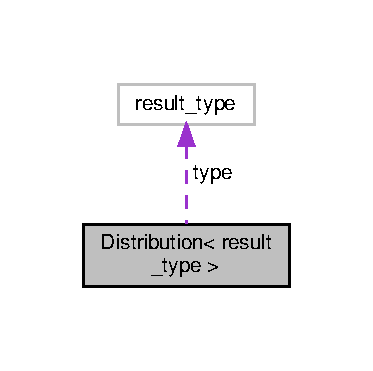
\includegraphics[width=179pt]{class_distribution__coll__graph}
\end{center}
\end{figure}
\subsection*{Public Member Functions}
\begin{DoxyCompactItemize}
\item 
\mbox{\Hypertarget{class_distribution_a5cd9af81203aa52556c25b34ba307b7d}\label{class_distribution_a5cd9af81203aa52556c25b34ba307b7d}} 
virtual result\+\_\+type \hyperlink{class_distribution_a5cd9af81203aa52556c25b34ba307b7d}{generate} ()=0
\begin{DoxyCompactList}\small\item\em Purely virtual generator of one random variable. \end{DoxyCompactList}\item 
\mbox{\Hypertarget{class_distribution_a827af71c147c83b35829e8b58ec0c089}\label{class_distribution_a827af71c147c83b35829e8b58ec0c089}} 
virtual std\+::vector$<$ result\+\_\+type $>$ \hyperlink{class_distribution_a827af71c147c83b35829e8b58ec0c089}{generate} (int n)=0
\begin{DoxyCompactList}\small\item\em Purely virtual generator of n random variables. \end{DoxyCompactList}\end{DoxyCompactItemize}
\subsection*{Private Attributes}
\begin{DoxyCompactItemize}
\item 
\mbox{\Hypertarget{class_distribution_a03f9b45f166879c67144cee48179c397}\label{class_distribution_a03f9b45f166879c67144cee48179c397}} 
result\+\_\+type \hyperlink{class_distribution_a03f9b45f166879c67144cee48179c397}{type}
\begin{DoxyCompactList}\small\item\em Type of output (either double or int)d. \end{DoxyCompactList}\end{DoxyCompactItemize}


\subsection{Detailed Description}
\subsubsection*{template$<$class result\+\_\+type$>$\newline
class Distribution$<$ result\+\_\+type $>$}

This is an abstract class for probability distributions 

The documentation for this class was generated from the following file\+:\begin{DoxyCompactItemize}
\item 
Distribution.\+hpp\end{DoxyCompactItemize}

\hypertarget{struct_exception}{}\section{Exception Struct Reference}
\label{struct_exception}\index{Exception@{Exception}}
\subsection*{Public Member Functions}
\begin{DoxyCompactItemize}
\item 
\mbox{\Hypertarget{struct_exception_a1799400f70924aba093edbc6f2ba6bfe}\label{struct_exception_a1799400f70924aba093edbc6f2ba6bfe}} 
{\bfseries Exception} (const std\+::string \&mesg)
\item 
\mbox{\Hypertarget{struct_exception_a19be342664e9da07334b8fbe7a253909}\label{struct_exception_a19be342664e9da07334b8fbe7a253909}} 
const std\+::string \& {\bfseries what} ()
\end{DoxyCompactItemize}
\subsection*{Public Attributes}
\begin{DoxyCompactItemize}
\item 
\mbox{\Hypertarget{struct_exception_ab13c042e7d550445aa548240ee2ed3e2}\label{struct_exception_ab13c042e7d550445aa548240ee2ed3e2}} 
std\+::string {\bfseries mesg}
\end{DoxyCompactItemize}


The documentation for this struct was generated from the following file\+:\begin{DoxyCompactItemize}
\item 
Exception.\+hpp\end{DoxyCompactItemize}

\hypertarget{class_exponential}{}\section{Exponential Class Reference}
\label{class_exponential}\index{Exponential@{Exponential}}


{\ttfamily \#include $<$Exponential.\+hpp$>$}



Inheritance diagram for Exponential\+:\nopagebreak
\begin{figure}[H]
\begin{center}
\leavevmode
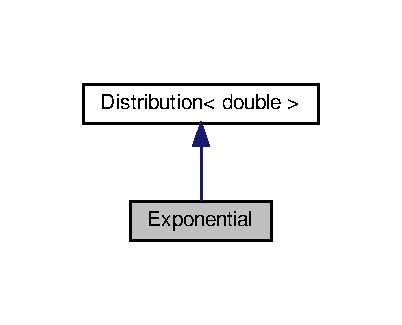
\includegraphics[width=193pt]{class_exponential__inherit__graph}
\end{center}
\end{figure}


Collaboration diagram for Exponential\+:\nopagebreak
\begin{figure}[H]
\begin{center}
\leavevmode
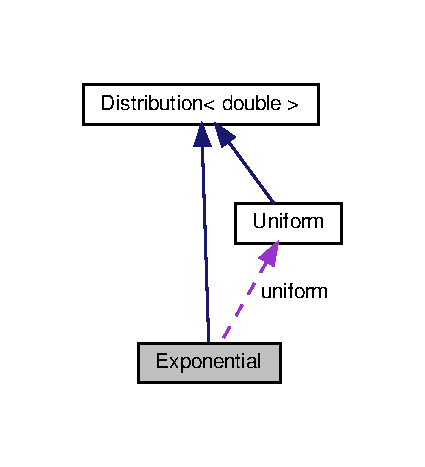
\includegraphics[width=204pt]{class_exponential__coll__graph}
\end{center}
\end{figure}
\subsection*{Public Member Functions}
\begin{DoxyCompactItemize}
\item 
\mbox{\Hypertarget{class_exponential_abc75eaef5b5f89656c4aa406aceb3c27}\label{class_exponential_abc75eaef5b5f89656c4aa406aceb3c27}} 
\hyperlink{class_exponential_abc75eaef5b5f89656c4aa406aceb3c27}{Exponential} ()
\begin{DoxyCompactList}\small\item\em Default constructor with rate set to 1.\+0. \end{DoxyCompactList}\item 
\mbox{\Hypertarget{class_exponential_a32dd612030caf5924c498a73f1fc72e8}\label{class_exponential_a32dd612030caf5924c498a73f1fc72e8}} 
\hyperlink{class_exponential_a32dd612030caf5924c498a73f1fc72e8}{Exponential} (double rate)
\begin{DoxyCompactList}\small\item\em Overloaded constructor with given rate lambda. \end{DoxyCompactList}\item 
\mbox{\Hypertarget{class_exponential_adf6d38352839ea9d7a15b2b98ed98a76}\label{class_exponential_adf6d38352839ea9d7a15b2b98ed98a76}} 
double \hyperlink{class_exponential_adf6d38352839ea9d7a15b2b98ed98a76}{get\+\_\+lambda} ()
\begin{DoxyCompactList}\small\item\em Returns rate. \end{DoxyCompactList}\item 
\mbox{\Hypertarget{class_exponential_ac7846dc0581e84750960825ad9ce4946}\label{class_exponential_ac7846dc0581e84750960825ad9ce4946}} 
double \hyperlink{class_exponential_ac7846dc0581e84750960825ad9ce4946}{generate} () override
\begin{DoxyCompactList}\small\item\em Generates one exponential random variable. \end{DoxyCompactList}\item 
\mbox{\Hypertarget{class_exponential_a10a4143f519e73772be2e766cda5bfea}\label{class_exponential_a10a4143f519e73772be2e766cda5bfea}} 
std\+::vector$<$ double $>$ \hyperlink{class_exponential_a10a4143f519e73772be2e766cda5bfea}{generate} (int n) override
\begin{DoxyCompactList}\small\item\em Generates n exponential random variables. \end{DoxyCompactList}\end{DoxyCompactItemize}
\subsection*{Private Attributes}
\begin{DoxyCompactItemize}
\item 
\mbox{\Hypertarget{class_exponential_aa3770de1a84c5669672eb5ff4f5f26b0}\label{class_exponential_aa3770de1a84c5669672eb5ff4f5f26b0}} 
\hyperlink{class_uniform}{Uniform} \hyperlink{class_exponential_aa3770de1a84c5669672eb5ff4f5f26b0}{uniform}
\begin{DoxyCompactList}\small\item\em \hyperlink{class_uniform}{Uniform} distribution used to generate normal random samples. \end{DoxyCompactList}\item 
\mbox{\Hypertarget{class_exponential_a2a48e288e649ddda226027379d0ce304}\label{class_exponential_a2a48e288e649ddda226027379d0ce304}} 
double \hyperlink{class_exponential_a2a48e288e649ddda226027379d0ce304}{lambda}
\begin{DoxyCompactList}\small\item\em Rate of the distribution. \end{DoxyCompactList}\end{DoxyCompactItemize}


\subsection{Detailed Description}
This is the class of exponential distributions. 

The documentation for this class was generated from the following files\+:\begin{DoxyCompactItemize}
\item 
Exponential.\+hpp\item 
Exponential.\+cpp\end{DoxyCompactItemize}

\hypertarget{class_geometric}{}\section{Geometric Class Reference}
\label{class_geometric}\index{Geometric@{Geometric}}


{\ttfamily \#include $<$Geometric.\+hpp$>$}



Inheritance diagram for Geometric\+:\nopagebreak
\begin{figure}[H]
\begin{center}
\leavevmode
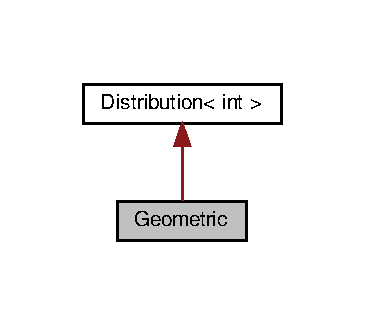
\includegraphics[width=175pt]{class_geometric__inherit__graph}
\end{center}
\end{figure}


Collaboration diagram for Geometric\+:\nopagebreak
\begin{figure}[H]
\begin{center}
\leavevmode
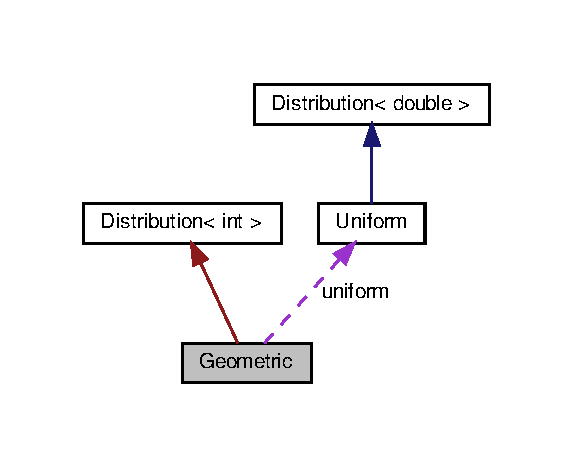
\includegraphics[width=275pt]{class_geometric__coll__graph}
\end{center}
\end{figure}
\subsection*{Public Member Functions}
\begin{DoxyCompactItemize}
\item 
\mbox{\Hypertarget{class_geometric_a741e184fee4d9abdeb2f565870eba117}\label{class_geometric_a741e184fee4d9abdeb2f565870eba117}} 
\hyperlink{class_geometric_a741e184fee4d9abdeb2f565870eba117}{Geometric} ()
\begin{DoxyCompactList}\small\item\em Default constructor with probability equal to 0.\+5. \end{DoxyCompactList}\item 
\mbox{\Hypertarget{class_geometric_a4e85b6271700782d644f56c5b90b4966}\label{class_geometric_a4e85b6271700782d644f56c5b90b4966}} 
\hyperlink{class_geometric_a4e85b6271700782d644f56c5b90b4966}{Geometric} (double p)
\begin{DoxyCompactList}\small\item\em Overloaded constructor taking another probability of success. \end{DoxyCompactList}\item 
\mbox{\Hypertarget{class_geometric_a486dd9216795ae5ecd3579598c62632c}\label{class_geometric_a486dd9216795ae5ecd3579598c62632c}} 
double \hyperlink{class_geometric_a486dd9216795ae5ecd3579598c62632c}{get\+\_\+probability} ()
\begin{DoxyCompactList}\small\item\em Returns probability of success. \end{DoxyCompactList}\item 
\mbox{\Hypertarget{class_geometric_a248e4a0a34c8681a5b3b889a4896a863}\label{class_geometric_a248e4a0a34c8681a5b3b889a4896a863}} 
int \hyperlink{class_geometric_a248e4a0a34c8681a5b3b889a4896a863}{generate} () override
\begin{DoxyCompactList}\small\item\em Generates one geometric random variable. \end{DoxyCompactList}\item 
\mbox{\Hypertarget{class_geometric_af1a6be5d5c92415648017a7e5eb87ecd}\label{class_geometric_af1a6be5d5c92415648017a7e5eb87ecd}} 
std\+::vector$<$ int $>$ \hyperlink{class_geometric_af1a6be5d5c92415648017a7e5eb87ecd}{generate} (int n) override
\begin{DoxyCompactList}\small\item\em Generates n geometric random variables. \end{DoxyCompactList}\end{DoxyCompactItemize}
\subsection*{Private Attributes}
\begin{DoxyCompactItemize}
\item 
\mbox{\Hypertarget{class_geometric_a8cf85792786df62248c0245bab9c6d28}\label{class_geometric_a8cf85792786df62248c0245bab9c6d28}} 
\hyperlink{class_uniform}{Uniform} \hyperlink{class_geometric_a8cf85792786df62248c0245bab9c6d28}{uniform}
\begin{DoxyCompactList}\small\item\em \hyperlink{class_uniform}{Uniform} distribution used to generate normal random samples. \end{DoxyCompactList}\item 
\mbox{\Hypertarget{class_geometric_abb5f3ad35a83e34e4ea139af69f13fe8}\label{class_geometric_abb5f3ad35a83e34e4ea139af69f13fe8}} 
double \hyperlink{class_geometric_abb5f3ad35a83e34e4ea139af69f13fe8}{probability}
\begin{DoxyCompactList}\small\item\em Probability of success for each trial. \end{DoxyCompactList}\end{DoxyCompactItemize}
\subsection*{Additional Inherited Members}


\subsection{Detailed Description}
This is the class of geometric distributions. It is defined as the number of failures before success so has support \{0, 1, 2, ... \} 

The documentation for this class was generated from the following files\+:\begin{DoxyCompactItemize}
\item 
Geometric.\+hpp\item 
Geometric.\+cpp\end{DoxyCompactItemize}

\hypertarget{class_moments}{}\section{Moments Class Reference}
\label{class_moments}\index{Moments@{Moments}}
\subsection*{Public Member Functions}
\begin{DoxyCompactItemize}
\item 
\mbox{\Hypertarget{class_moments_af8f51e719b3565253eb67a7fd7667502}\label{class_moments_af8f51e719b3565253eb67a7fd7667502}} 
{\bfseries Moments} (int order, bool centered, double($\ast$f)(std\+::vector$<$ double $>$ \&random\+\_\+vector))
\item 
\mbox{\Hypertarget{class_moments_a1dbde91cd8e38936ebe0361b71c78967}\label{class_moments_a1dbde91cd8e38936ebe0361b71c78967}} 
void {\bfseries set\+\_\+p} (int order)
\item 
\mbox{\Hypertarget{class_moments_a25155c9efacd719224154c3b69dea863}\label{class_moments_a25155c9efacd719224154c3b69dea863}} 
int {\bfseries get\+\_\+p} ()
\item 
\mbox{\Hypertarget{class_moments_ac5549fdcf86889e7cfc7527801279486}\label{class_moments_ac5549fdcf86889e7cfc7527801279486}} 
void {\bfseries set\+\_\+central} (bool centered)
\item 
\mbox{\Hypertarget{class_moments_a26d12173d77025d2542765d317df3f13}\label{class_moments_a26d12173d77025d2542765d317df3f13}} 
bool {\bfseries get\+\_\+central} ()
\item 
\mbox{\Hypertarget{class_moments_a054c3ebc912c0510ccb4d80cd3741568}\label{class_moments_a054c3ebc912c0510ccb4d80cd3741568}} 
void {\bfseries set\+\_\+function} (double($\ast$f)(std\+::vector$<$ double $>$ \&random\+\_\+vector))
\item 
\mbox{\Hypertarget{class_moments_af2f6c5757bf3f80b50997e21d386ccf9}\label{class_moments_af2f6c5757bf3f80b50997e21d386ccf9}} 
double {\bfseries calculate} ()
\end{DoxyCompactItemize}
\subsection*{Private Attributes}
\begin{DoxyCompactItemize}
\item 
\mbox{\Hypertarget{class_moments_a7024e63f29ef5003294e24ba89af914a}\label{class_moments_a7024e63f29ef5003294e24ba89af914a}} 
int {\bfseries p}
\item 
\mbox{\Hypertarget{class_moments_a0653b35a365550a072f171c47627a7a3}\label{class_moments_a0653b35a365550a072f171c47627a7a3}} 
bool {\bfseries central}
\item 
\mbox{\Hypertarget{class_moments_ac6fa678f67e41cba1b7c6d8846e9dd8f}\label{class_moments_ac6fa678f67e41cba1b7c6d8846e9dd8f}} 
double($\ast$ {\bfseries user\+\_\+defined\+\_\+function} )(std\+::vector$<$ double $>$ \&random\+\_\+vec)
\end{DoxyCompactItemize}


The documentation for this class was generated from the following files\+:\begin{DoxyCompactItemize}
\item 
Moments.\+hpp\item 
Moments.\+cpp\end{DoxyCompactItemize}

\hypertarget{class_normal}{}\section{Normal Class Reference}
\label{class_normal}\index{Normal@{Normal}}


{\ttfamily \#include $<$Normal.\+hpp$>$}



Inheritance diagram for Normal\+:\nopagebreak
\begin{figure}[H]
\begin{center}
\leavevmode
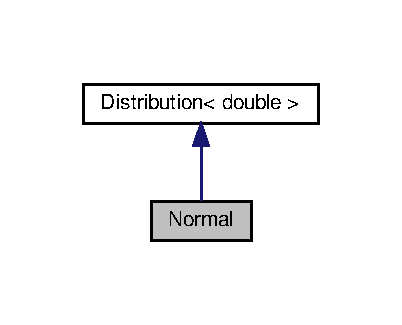
\includegraphics[width=193pt]{class_normal__inherit__graph}
\end{center}
\end{figure}


Collaboration diagram for Normal\+:\nopagebreak
\begin{figure}[H]
\begin{center}
\leavevmode
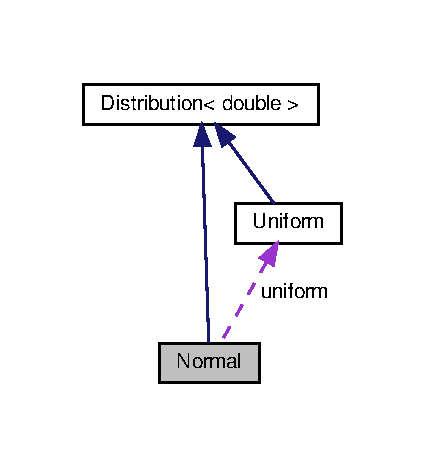
\includegraphics[width=204pt]{class_normal__coll__graph}
\end{center}
\end{figure}
\subsection*{Public Member Functions}
\begin{DoxyCompactItemize}
\item 
\mbox{\Hypertarget{class_normal_af62e51ec40dc2eedc3b9ca49ebdc7197}\label{class_normal_af62e51ec40dc2eedc3b9ca49ebdc7197}} 
\hyperlink{class_normal_af62e51ec40dc2eedc3b9ca49ebdc7197}{Normal} ()
\begin{DoxyCompactList}\small\item\em Default constructor with mean 0 and standard deviation 1. \end{DoxyCompactList}\item 
\mbox{\Hypertarget{class_normal_aa1c65330d29f9d34a3c35e01371a5a0c}\label{class_normal_aa1c65330d29f9d34a3c35e01371a5a0c}} 
\hyperlink{class_normal_aa1c65330d29f9d34a3c35e01371a5a0c}{Normal} (double mean, double std)
\begin{DoxyCompactList}\small\item\em Overloaded constructor taking mean and standard deviation. \end{DoxyCompactList}\item 
\mbox{\Hypertarget{class_normal_aa28b93c40d959490fdb7e944cfb53ce5}\label{class_normal_aa28b93c40d959490fdb7e944cfb53ce5}} 
double \hyperlink{class_normal_aa28b93c40d959490fdb7e944cfb53ce5}{get\+\_\+mu} ()
\begin{DoxyCompactList}\small\item\em Returns mean. \end{DoxyCompactList}\item 
\mbox{\Hypertarget{class_normal_ab0fb264168e878f12d2a9eddbfefda79}\label{class_normal_ab0fb264168e878f12d2a9eddbfefda79}} 
double \hyperlink{class_normal_ab0fb264168e878f12d2a9eddbfefda79}{get\+\_\+sigma} ()
\begin{DoxyCompactList}\small\item\em Returns standard deviation. \end{DoxyCompactList}\item 
\mbox{\Hypertarget{class_normal_ace26d5def9f3a3fb469408a4f38ad37d}\label{class_normal_ace26d5def9f3a3fb469408a4f38ad37d}} 
double \hyperlink{class_normal_ace26d5def9f3a3fb469408a4f38ad37d}{generate} () override
\begin{DoxyCompactList}\small\item\em Generate one normal random variable. \end{DoxyCompactList}\item 
\mbox{\Hypertarget{class_normal_a0618904d563dbb1baae5441abc8677a2}\label{class_normal_a0618904d563dbb1baae5441abc8677a2}} 
std\+::vector$<$ double $>$ \hyperlink{class_normal_a0618904d563dbb1baae5441abc8677a2}{generate} (int n) override
\begin{DoxyCompactList}\small\item\em Generate n normal random variables. \end{DoxyCompactList}\end{DoxyCompactItemize}
\subsection*{Private Attributes}
\begin{DoxyCompactItemize}
\item 
\mbox{\Hypertarget{class_normal_a206a8e2aeaea2ed71218fed4af5cac22}\label{class_normal_a206a8e2aeaea2ed71218fed4af5cac22}} 
\hyperlink{class_uniform}{Uniform} \hyperlink{class_normal_a206a8e2aeaea2ed71218fed4af5cac22}{uniform}
\begin{DoxyCompactList}\small\item\em \hyperlink{class_uniform}{Uniform} distribution used to generate normal random samples. \end{DoxyCompactList}\item 
\mbox{\Hypertarget{class_normal_ae96fa398a2a81b7c9b6fa620591be505}\label{class_normal_ae96fa398a2a81b7c9b6fa620591be505}} 
double \hyperlink{class_normal_ae96fa398a2a81b7c9b6fa620591be505}{mu}
\begin{DoxyCompactList}\small\item\em Mean of the normal distribution. \end{DoxyCompactList}\item 
\mbox{\Hypertarget{class_normal_a21090738bd2f532e36026d9536e565af}\label{class_normal_a21090738bd2f532e36026d9536e565af}} 
double \hyperlink{class_normal_a21090738bd2f532e36026d9536e565af}{sigma}
\begin{DoxyCompactList}\small\item\em Standard deviation of the normal distribution. \end{DoxyCompactList}\end{DoxyCompactItemize}


\subsection{Detailed Description}
This is a class of one-\/dimensional normal (Gaussian) distributions. 

The documentation for this class was generated from the following files\+:\begin{DoxyCompactItemize}
\item 
Normal.\+hpp\item 
Normal.\+cpp\end{DoxyCompactItemize}

\hypertarget{struct_printer}{}\section{Printer Struct Reference}
\label{struct_printer}\index{Printer@{Printer}}
\subsection*{Public Member Functions}
\begin{DoxyCompactItemize}
\item 
\mbox{\Hypertarget{struct_printer_a48a978e4d866ed8462b5aae4fa238b7c}\label{struct_printer_a48a978e4d866ed8462b5aae4fa238b7c}} 
{\bfseries Printer} (std\+::ostream \&os)
\item 
\mbox{\Hypertarget{struct_printer_ae556fdf28494ef0e8c46d5bf8ce59899}\label{struct_printer_ae556fdf28494ef0e8c46d5bf8ce59899}} 
{\footnotesize template$<$typename T $>$ }\\void {\bfseries operator()} (const T \&obj)
\end{DoxyCompactItemize}
\subsection*{Public Attributes}
\begin{DoxyCompactItemize}
\item 
\mbox{\Hypertarget{struct_printer_a96e24dc8390d3aba4993780282b330ae}\label{struct_printer_a96e24dc8390d3aba4993780282b330ae}} 
std\+::ostream \& {\bfseries os}
\end{DoxyCompactItemize}


The documentation for this struct was generated from the following file\+:\begin{DoxyCompactItemize}
\item 
main.\+cpp\end{DoxyCompactItemize}

\hypertarget{structmatplotlibcpp_1_1select__npy__type}{}\section{matplotlibcpp\+:\+:select\+\_\+npy\+\_\+type$<$ T $>$ Struct Template Reference}
\label{structmatplotlibcpp_1_1select__npy__type}\index{matplotlibcpp\+::select\+\_\+npy\+\_\+type$<$ T $>$@{matplotlibcpp\+::select\+\_\+npy\+\_\+type$<$ T $>$}}
\subsection*{Static Public Attributes}
\begin{DoxyCompactItemize}
\item 
\mbox{\Hypertarget{structmatplotlibcpp_1_1select__npy__type_acbffa4e6e1d047b52e12330446816c9c}\label{structmatplotlibcpp_1_1select__npy__type_acbffa4e6e1d047b52e12330446816c9c}} 
static const N\+P\+Y\+\_\+\+T\+Y\+P\+ES {\bfseries type} = N\+P\+Y\+\_\+\+N\+O\+T\+Y\+PE
\end{DoxyCompactItemize}


The documentation for this struct was generated from the following file\+:\begin{DoxyCompactItemize}
\item 
matplotlibcpp.\+h\end{DoxyCompactItemize}

\hypertarget{structmatplotlibcpp_1_1select__npy__type_3_01bool_01_4}{}\section{matplotlibcpp\+:\+:select\+\_\+npy\+\_\+type$<$ bool $>$ Struct Template Reference}
\label{structmatplotlibcpp_1_1select__npy__type_3_01bool_01_4}\index{matplotlibcpp\+::select\+\_\+npy\+\_\+type$<$ bool $>$@{matplotlibcpp\+::select\+\_\+npy\+\_\+type$<$ bool $>$}}
\subsection*{Static Public Attributes}
\begin{DoxyCompactItemize}
\item 
\mbox{\Hypertarget{structmatplotlibcpp_1_1select__npy__type_3_01bool_01_4_a79dc3db61a3b0f4796a29d067d5dd374}\label{structmatplotlibcpp_1_1select__npy__type_3_01bool_01_4_a79dc3db61a3b0f4796a29d067d5dd374}} 
static const N\+P\+Y\+\_\+\+T\+Y\+P\+ES {\bfseries type} = N\+P\+Y\+\_\+\+B\+O\+OL
\end{DoxyCompactItemize}


The documentation for this struct was generated from the following file\+:\begin{DoxyCompactItemize}
\item 
matplotlibcpp.\+h\end{DoxyCompactItemize}

\hypertarget{structmatplotlibcpp_1_1select__npy__type_3_01double_01_4}{}\section{matplotlibcpp\+:\+:select\+\_\+npy\+\_\+type$<$ double $>$ Struct Template Reference}
\label{structmatplotlibcpp_1_1select__npy__type_3_01double_01_4}\index{matplotlibcpp\+::select\+\_\+npy\+\_\+type$<$ double $>$@{matplotlibcpp\+::select\+\_\+npy\+\_\+type$<$ double $>$}}
\subsection*{Static Public Attributes}
\begin{DoxyCompactItemize}
\item 
\mbox{\Hypertarget{structmatplotlibcpp_1_1select__npy__type_3_01double_01_4_a939edaf81fedb879c8c90ad13c98a709}\label{structmatplotlibcpp_1_1select__npy__type_3_01double_01_4_a939edaf81fedb879c8c90ad13c98a709}} 
static const N\+P\+Y\+\_\+\+T\+Y\+P\+ES {\bfseries type} = N\+P\+Y\+\_\+\+D\+O\+U\+B\+LE
\end{DoxyCompactItemize}


The documentation for this struct was generated from the following file\+:\begin{DoxyCompactItemize}
\item 
matplotlibcpp.\+h\end{DoxyCompactItemize}

\hypertarget{structmatplotlibcpp_1_1select__npy__type_3_01float_01_4}{}\section{matplotlibcpp\+:\+:select\+\_\+npy\+\_\+type$<$ float $>$ Struct Template Reference}
\label{structmatplotlibcpp_1_1select__npy__type_3_01float_01_4}\index{matplotlibcpp\+::select\+\_\+npy\+\_\+type$<$ float $>$@{matplotlibcpp\+::select\+\_\+npy\+\_\+type$<$ float $>$}}
\subsection*{Static Public Attributes}
\begin{DoxyCompactItemize}
\item 
\mbox{\Hypertarget{structmatplotlibcpp_1_1select__npy__type_3_01float_01_4_a7bca025a3f0cb143e566e0f575bf7f6b}\label{structmatplotlibcpp_1_1select__npy__type_3_01float_01_4_a7bca025a3f0cb143e566e0f575bf7f6b}} 
static const N\+P\+Y\+\_\+\+T\+Y\+P\+ES {\bfseries type} = N\+P\+Y\+\_\+\+F\+L\+O\+AT
\end{DoxyCompactItemize}


The documentation for this struct was generated from the following file\+:\begin{DoxyCompactItemize}
\item 
matplotlibcpp.\+h\end{DoxyCompactItemize}

\hypertarget{structmatplotlibcpp_1_1select__npy__type_3_01int16__t_01_4}{}\section{matplotlibcpp\+:\+:select\+\_\+npy\+\_\+type$<$ int16\+\_\+t $>$ Struct Template Reference}
\label{structmatplotlibcpp_1_1select__npy__type_3_01int16__t_01_4}\index{matplotlibcpp\+::select\+\_\+npy\+\_\+type$<$ int16\+\_\+t $>$@{matplotlibcpp\+::select\+\_\+npy\+\_\+type$<$ int16\+\_\+t $>$}}
\subsection*{Static Public Attributes}
\begin{DoxyCompactItemize}
\item 
\mbox{\Hypertarget{structmatplotlibcpp_1_1select__npy__type_3_01int16__t_01_4_aa7e1803c594ccc58c2cd4c8818d5a158}\label{structmatplotlibcpp_1_1select__npy__type_3_01int16__t_01_4_aa7e1803c594ccc58c2cd4c8818d5a158}} 
static const N\+P\+Y\+\_\+\+T\+Y\+P\+ES {\bfseries type} = N\+P\+Y\+\_\+\+S\+H\+O\+RT
\end{DoxyCompactItemize}


The documentation for this struct was generated from the following file\+:\begin{DoxyCompactItemize}
\item 
matplotlibcpp.\+h\end{DoxyCompactItemize}

\hypertarget{structmatplotlibcpp_1_1select__npy__type_3_01int32__t_01_4}{}\section{matplotlibcpp\+:\+:select\+\_\+npy\+\_\+type$<$ int32\+\_\+t $>$ Struct Template Reference}
\label{structmatplotlibcpp_1_1select__npy__type_3_01int32__t_01_4}\index{matplotlibcpp\+::select\+\_\+npy\+\_\+type$<$ int32\+\_\+t $>$@{matplotlibcpp\+::select\+\_\+npy\+\_\+type$<$ int32\+\_\+t $>$}}
\subsection*{Static Public Attributes}
\begin{DoxyCompactItemize}
\item 
\mbox{\Hypertarget{structmatplotlibcpp_1_1select__npy__type_3_01int32__t_01_4_abcfd0c3dc5d5e92575c04747315cb4d5}\label{structmatplotlibcpp_1_1select__npy__type_3_01int32__t_01_4_abcfd0c3dc5d5e92575c04747315cb4d5}} 
static const N\+P\+Y\+\_\+\+T\+Y\+P\+ES {\bfseries type} = N\+P\+Y\+\_\+\+I\+NT
\end{DoxyCompactItemize}


The documentation for this struct was generated from the following file\+:\begin{DoxyCompactItemize}
\item 
matplotlibcpp.\+h\end{DoxyCompactItemize}

\hypertarget{structmatplotlibcpp_1_1select__npy__type_3_01int64__t_01_4}{}\section{matplotlibcpp\+:\+:select\+\_\+npy\+\_\+type$<$ int64\+\_\+t $>$ Struct Template Reference}
\label{structmatplotlibcpp_1_1select__npy__type_3_01int64__t_01_4}\index{matplotlibcpp\+::select\+\_\+npy\+\_\+type$<$ int64\+\_\+t $>$@{matplotlibcpp\+::select\+\_\+npy\+\_\+type$<$ int64\+\_\+t $>$}}
\subsection*{Static Public Attributes}
\begin{DoxyCompactItemize}
\item 
\mbox{\Hypertarget{structmatplotlibcpp_1_1select__npy__type_3_01int64__t_01_4_a0d20ea35e520ad9381aca3c173f3f02d}\label{structmatplotlibcpp_1_1select__npy__type_3_01int64__t_01_4_a0d20ea35e520ad9381aca3c173f3f02d}} 
static const N\+P\+Y\+\_\+\+T\+Y\+P\+ES {\bfseries type} = N\+P\+Y\+\_\+\+I\+N\+T64
\end{DoxyCompactItemize}


The documentation for this struct was generated from the following file\+:\begin{DoxyCompactItemize}
\item 
matplotlibcpp.\+h\end{DoxyCompactItemize}

\hypertarget{structmatplotlibcpp_1_1select__npy__type_3_01int8__t_01_4}{}\section{matplotlibcpp\+:\+:select\+\_\+npy\+\_\+type$<$ int8\+\_\+t $>$ Struct Template Reference}
\label{structmatplotlibcpp_1_1select__npy__type_3_01int8__t_01_4}\index{matplotlibcpp\+::select\+\_\+npy\+\_\+type$<$ int8\+\_\+t $>$@{matplotlibcpp\+::select\+\_\+npy\+\_\+type$<$ int8\+\_\+t $>$}}
\subsection*{Static Public Attributes}
\begin{DoxyCompactItemize}
\item 
\mbox{\Hypertarget{structmatplotlibcpp_1_1select__npy__type_3_01int8__t_01_4_a74836a19458ed32ca8948a4337364eae}\label{structmatplotlibcpp_1_1select__npy__type_3_01int8__t_01_4_a74836a19458ed32ca8948a4337364eae}} 
static const N\+P\+Y\+\_\+\+T\+Y\+P\+ES {\bfseries type} = N\+P\+Y\+\_\+\+I\+N\+T8
\end{DoxyCompactItemize}


The documentation for this struct was generated from the following file\+:\begin{DoxyCompactItemize}
\item 
matplotlibcpp.\+h\end{DoxyCompactItemize}

\hypertarget{structmatplotlibcpp_1_1select__npy__type_3_01uint16__t_01_4}{}\section{matplotlibcpp\+:\+:select\+\_\+npy\+\_\+type$<$ uint16\+\_\+t $>$ Struct Template Reference}
\label{structmatplotlibcpp_1_1select__npy__type_3_01uint16__t_01_4}\index{matplotlibcpp\+::select\+\_\+npy\+\_\+type$<$ uint16\+\_\+t $>$@{matplotlibcpp\+::select\+\_\+npy\+\_\+type$<$ uint16\+\_\+t $>$}}
\subsection*{Static Public Attributes}
\begin{DoxyCompactItemize}
\item 
\mbox{\Hypertarget{structmatplotlibcpp_1_1select__npy__type_3_01uint16__t_01_4_aca209b33cc0bcaad16c01bff097a075f}\label{structmatplotlibcpp_1_1select__npy__type_3_01uint16__t_01_4_aca209b33cc0bcaad16c01bff097a075f}} 
static const N\+P\+Y\+\_\+\+T\+Y\+P\+ES {\bfseries type} = N\+P\+Y\+\_\+\+U\+S\+H\+O\+RT
\end{DoxyCompactItemize}


The documentation for this struct was generated from the following file\+:\begin{DoxyCompactItemize}
\item 
matplotlibcpp.\+h\end{DoxyCompactItemize}

\hypertarget{structmatplotlibcpp_1_1select__npy__type_3_01uint32__t_01_4}{}\section{matplotlibcpp\+:\+:select\+\_\+npy\+\_\+type$<$ uint32\+\_\+t $>$ Struct Template Reference}
\label{structmatplotlibcpp_1_1select__npy__type_3_01uint32__t_01_4}\index{matplotlibcpp\+::select\+\_\+npy\+\_\+type$<$ uint32\+\_\+t $>$@{matplotlibcpp\+::select\+\_\+npy\+\_\+type$<$ uint32\+\_\+t $>$}}
\subsection*{Static Public Attributes}
\begin{DoxyCompactItemize}
\item 
\mbox{\Hypertarget{structmatplotlibcpp_1_1select__npy__type_3_01uint32__t_01_4_a21b0fbd17b661ef512cc1c3c728dfa60}\label{structmatplotlibcpp_1_1select__npy__type_3_01uint32__t_01_4_a21b0fbd17b661ef512cc1c3c728dfa60}} 
static const N\+P\+Y\+\_\+\+T\+Y\+P\+ES {\bfseries type} = N\+P\+Y\+\_\+\+U\+L\+O\+NG
\end{DoxyCompactItemize}


The documentation for this struct was generated from the following file\+:\begin{DoxyCompactItemize}
\item 
matplotlibcpp.\+h\end{DoxyCompactItemize}

\hypertarget{structmatplotlibcpp_1_1select__npy__type_3_01uint64__t_01_4}{}\section{matplotlibcpp\+:\+:select\+\_\+npy\+\_\+type$<$ uint64\+\_\+t $>$ Struct Template Reference}
\label{structmatplotlibcpp_1_1select__npy__type_3_01uint64__t_01_4}\index{matplotlibcpp\+::select\+\_\+npy\+\_\+type$<$ uint64\+\_\+t $>$@{matplotlibcpp\+::select\+\_\+npy\+\_\+type$<$ uint64\+\_\+t $>$}}
\subsection*{Static Public Attributes}
\begin{DoxyCompactItemize}
\item 
\mbox{\Hypertarget{structmatplotlibcpp_1_1select__npy__type_3_01uint64__t_01_4_a8d5871452f90ff04452f0416bee54fca}\label{structmatplotlibcpp_1_1select__npy__type_3_01uint64__t_01_4_a8d5871452f90ff04452f0416bee54fca}} 
static const N\+P\+Y\+\_\+\+T\+Y\+P\+ES {\bfseries type} = N\+P\+Y\+\_\+\+U\+I\+N\+T64
\end{DoxyCompactItemize}


The documentation for this struct was generated from the following file\+:\begin{DoxyCompactItemize}
\item 
matplotlibcpp.\+h\end{DoxyCompactItemize}

\hypertarget{structmatplotlibcpp_1_1select__npy__type_3_01uint8__t_01_4}{}\section{matplotlibcpp\+:\+:select\+\_\+npy\+\_\+type$<$ uint8\+\_\+t $>$ Struct Template Reference}
\label{structmatplotlibcpp_1_1select__npy__type_3_01uint8__t_01_4}\index{matplotlibcpp\+::select\+\_\+npy\+\_\+type$<$ uint8\+\_\+t $>$@{matplotlibcpp\+::select\+\_\+npy\+\_\+type$<$ uint8\+\_\+t $>$}}
\subsection*{Static Public Attributes}
\begin{DoxyCompactItemize}
\item 
\mbox{\Hypertarget{structmatplotlibcpp_1_1select__npy__type_3_01uint8__t_01_4_a6e80bfd252a69f14ff869c8b4fbb9e54}\label{structmatplotlibcpp_1_1select__npy__type_3_01uint8__t_01_4_a6e80bfd252a69f14ff869c8b4fbb9e54}} 
static const N\+P\+Y\+\_\+\+T\+Y\+P\+ES {\bfseries type} = N\+P\+Y\+\_\+\+U\+I\+N\+T8
\end{DoxyCompactItemize}


The documentation for this struct was generated from the following file\+:\begin{DoxyCompactItemize}
\item 
matplotlibcpp.\+h\end{DoxyCompactItemize}

\hypertarget{class_uniform}{}\section{Uniform Class Reference}
\label{class_uniform}\index{Uniform@{Uniform}}


{\ttfamily \#include $<$Uniform.\+hpp$>$}



Inheritance diagram for Uniform\+:\nopagebreak
\begin{figure}[H]
\begin{center}
\leavevmode
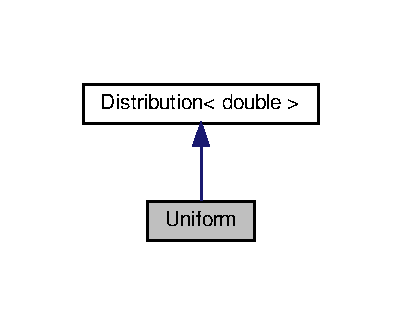
\includegraphics[width=193pt]{class_uniform__inherit__graph}
\end{center}
\end{figure}


Collaboration diagram for Uniform\+:\nopagebreak
\begin{figure}[H]
\begin{center}
\leavevmode
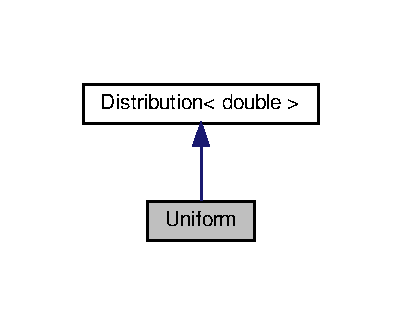
\includegraphics[width=193pt]{class_uniform__coll__graph}
\end{center}
\end{figure}
\subsection*{Public Member Functions}
\begin{DoxyCompactItemize}
\item 
\mbox{\Hypertarget{class_uniform_a55d4df320842397431ce1b57c43924e8}\label{class_uniform_a55d4df320842397431ce1b57c43924e8}} 
\hyperlink{class_uniform_a55d4df320842397431ce1b57c43924e8}{Uniform} ()
\begin{DoxyCompactList}\small\item\em Default constructor. \end{DoxyCompactList}\item 
\mbox{\Hypertarget{class_uniform_a9c9a8915fe92ac802a55dd3875045a73}\label{class_uniform_a9c9a8915fe92ac802a55dd3875045a73}} 
\hyperlink{class_uniform_a9c9a8915fe92ac802a55dd3875045a73}{Uniform} (double min, double max)
\begin{DoxyCompactList}\small\item\em Overloaded constructor taking minimum and maximum. \end{DoxyCompactList}\item 
\mbox{\Hypertarget{class_uniform_a82e17d9668c7a2463a533c8fea9b2222}\label{class_uniform_a82e17d9668c7a2463a533c8fea9b2222}} 
double \hyperlink{class_uniform_a82e17d9668c7a2463a533c8fea9b2222}{get\+\_\+a} ()
\begin{DoxyCompactList}\small\item\em Returns minimum. \end{DoxyCompactList}\item 
\mbox{\Hypertarget{class_uniform_a7bd95be60e4243b9b7157fa4fa32f8d9}\label{class_uniform_a7bd95be60e4243b9b7157fa4fa32f8d9}} 
double \hyperlink{class_uniform_a7bd95be60e4243b9b7157fa4fa32f8d9}{get\+\_\+b} ()
\begin{DoxyCompactList}\small\item\em Returns maximum. \end{DoxyCompactList}\item 
\mbox{\Hypertarget{class_uniform_ab9562a5945249b603a26f1c6e9be1091}\label{class_uniform_ab9562a5945249b603a26f1c6e9be1091}} 
double \hyperlink{class_uniform_ab9562a5945249b603a26f1c6e9be1091}{generate} () override
\begin{DoxyCompactList}\small\item\em Generate one uniform random variable. \end{DoxyCompactList}\item 
\mbox{\Hypertarget{class_uniform_a15f9f527e4e2dc35d1f0da34d9b21ed3}\label{class_uniform_a15f9f527e4e2dc35d1f0da34d9b21ed3}} 
std\+::vector$<$ double $>$ \hyperlink{class_uniform_a15f9f527e4e2dc35d1f0da34d9b21ed3}{generate} (int n) override
\begin{DoxyCompactList}\small\item\em Generate n uniform random variables. \end{DoxyCompactList}\end{DoxyCompactItemize}
\subsection*{Private Attributes}
\begin{DoxyCompactItemize}
\item 
\mbox{\Hypertarget{class_uniform_a7264c2617a82aaaf04b17fc3911368b9}\label{class_uniform_a7264c2617a82aaaf04b17fc3911368b9}} 
double \hyperlink{class_uniform_a7264c2617a82aaaf04b17fc3911368b9}{a}
\begin{DoxyCompactList}\small\item\em Minimum of the uniform distribution. \end{DoxyCompactList}\item 
\mbox{\Hypertarget{class_uniform_a6d556bd18b80242b58adfde0dd12e319}\label{class_uniform_a6d556bd18b80242b58adfde0dd12e319}} 
double \hyperlink{class_uniform_a6d556bd18b80242b58adfde0dd12e319}{b}
\begin{DoxyCompactList}\small\item\em Maximum of the uniform distribution. \end{DoxyCompactList}\end{DoxyCompactItemize}


\subsection{Detailed Description}
This is a class of continuous uniform distributions. 

The documentation for this class was generated from the following files\+:\begin{DoxyCompactItemize}
\item 
Uniform.\+hpp\item 
Uniform.\+cpp\end{DoxyCompactItemize}

\hypertarget{class_verify_c_l_t}{}\section{Verify\+C\+LT Class Reference}
\label{class_verify_c_l_t}\index{Verify\+C\+LT@{Verify\+C\+LT}}


Collaboration diagram for Verify\+C\+LT\+:
\nopagebreak
\begin{figure}[H]
\begin{center}
\leavevmode
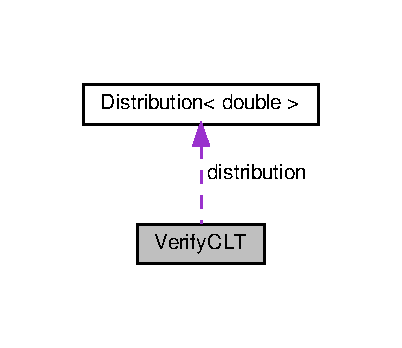
\includegraphics[width=193pt]{class_verify_c_l_t__coll__graph}
\end{center}
\end{figure}
\subsection*{Public Member Functions}
\begin{DoxyCompactItemize}
\item 
\mbox{\Hypertarget{class_verify_c_l_t_a74ff104685619dc300c4df913de8b784}\label{class_verify_c_l_t_a74ff104685619dc300c4df913de8b784}} 
void {\bfseries set\+\_\+num\+\_\+samples} (int n)
\item 
\mbox{\Hypertarget{class_verify_c_l_t_ac7b6d9e8c6fa5af0ec0a65d336079aab}\label{class_verify_c_l_t_ac7b6d9e8c6fa5af0ec0a65d336079aab}} 
int {\bfseries get\+\_\+num\+\_\+samples} ()
\item 
\mbox{\Hypertarget{class_verify_c_l_t_a001bc8b46a677aa50fc012de3959d8d1}\label{class_verify_c_l_t_a001bc8b46a677aa50fc012de3959d8d1}} 
void {\bfseries set\+\_\+num\+\_\+trials} (int n)
\item 
\mbox{\Hypertarget{class_verify_c_l_t_af14925645c905b040f32cd65fcd3fe14}\label{class_verify_c_l_t_af14925645c905b040f32cd65fcd3fe14}} 
int {\bfseries get\+\_\+num\+\_\+trials} ()
\item 
\mbox{\Hypertarget{class_verify_c_l_t_ad1ba3f5a9867ec43ade06ea58cb0c30e}\label{class_verify_c_l_t_ad1ba3f5a9867ec43ade06ea58cb0c30e}} 
void {\bfseries histogram} ()
\item 
\mbox{\Hypertarget{class_verify_c_l_t_a21c6be46ba54c7b9719dd84533210886}\label{class_verify_c_l_t_a21c6be46ba54c7b9719dd84533210886}} 
void {\bfseries qq\+\_\+plot} ()
\end{DoxyCompactItemize}
\subsection*{Private Attributes}
\begin{DoxyCompactItemize}
\item 
\mbox{\Hypertarget{class_verify_c_l_t_ac8a8074a0611cdafba6d6ca5d0a03c1d}\label{class_verify_c_l_t_ac8a8074a0611cdafba6d6ca5d0a03c1d}} 
int {\bfseries num\+\_\+samples}
\item 
\mbox{\Hypertarget{class_verify_c_l_t_ad1f356e44fb1043662c49851dd1af325}\label{class_verify_c_l_t_ad1f356e44fb1043662c49851dd1af325}} 
int {\bfseries num\+\_\+trials}
\item 
\mbox{\Hypertarget{class_verify_c_l_t_a25804188d54b373ba842b94778a2bf3e}\label{class_verify_c_l_t_a25804188d54b373ba842b94778a2bf3e}} 
\hyperlink{class_distribution}{Distribution}$<$ double $>$ $\ast$ {\bfseries distribution}
\end{DoxyCompactItemize}


The documentation for this class was generated from the following files\+:\begin{DoxyCompactItemize}
\item 
Verify\+C\+L\+T.\+hpp\item 
Verify\+C\+L\+T.\+cpp\end{DoxyCompactItemize}

%--- End generated contents ---

% Index
\backmatter
\newpage
\phantomsection
\clearemptydoublepage
\addcontentsline{toc}{chapter}{Index}
\printindex

\end{document}
